\documentclass[pdftex,letterpaper,11pt]{article}%
\usepackage[export]{adjustbox}
\usepackage{multirow}
\usepackage[arabicsections]{dpugatex}
%\usepackage{dpppl}
%\usepackage{lscape}
\usepackage{pdflscape}
\usepackage{longtable}


\usepackage{tikz}

\usepackage[british]{babel}
\usepackage{amssymb,amsmath,warpcol,url,ctable,multirow,caption,threeparttable,float,soul,gensymb}
%\usepackage[noend]{algpseudocode}
\makeatletter
\def\BState{\State\hskip-\ALG@thistlm}
\makeatother


\usepackage{subcaption}


\usepackage{xcolor,colortbl}%Per colorejar cel·les de les taules
\definecolor{verylightgray}{gray}{0.90}
\newcommand{\verylightgray}[1]{\cellcolor{verylightgray}#1}


\usepackage{arydshln} %Per dashed lines
\setlength\dashlinedash{1.5pt}
\setlength\dashlinegap{2.5pt}
\setlength\arrayrulewidth{0.8pt}

\usepackage[utf8]{inputenc}
\usepackage{eurosym}
\usepackage{soul}
\setstcolor{red} % Tatxat vermell pel text a eliminar!!!!
\definecolor{lightgreen}{rgb}{0.564706,0.933333,0.564706}
\newcommand{\miquel}[1]{{\sethlcolor{lightgreen} \hl{#1}} } % To highlight with light green Miquel's comments.
\soulregister\citet7 % These \soulregister commands allow us to avoid problems between soul functions (\hl, \st, ...) and these other functions (\citet,\citep,\ref,\footnote, ...). Include more if it is necessary.
\soulregister\citep7
\soulregister\cite7
\soulregister\ref7
\soulregister\footnote7
\soulregister\textit7
\soulregister\textbf7
\soulregister\textsc7
\soulregister\`7 % for open accents.
\soulregister\'7 % for closed accents.
\soulregister\% 7 % for \%age symbol
\usepackage{tabularx,tabulary}
\usepackage[osf]{mathpazo} % Amb aquest paquet faig ús de la lletra Palatino, la que fan servir Puga, Duranton et al. Amb l'opció [osf] la numeració és "old fashion", però és incompatible amb un títol en negreta i small caps (desapareixen les small caps!). Per tant, per ara opto per NO aplicar aquesta opció.
\usepackage[abs]{overpic}

\usepackage{hyperref}
\definecolor{darkblue}{rgb}{0.0,0.0,0.3}
\hypersetup{colorlinks=true, breaklinks=true, citecolor= darkblue, linkcolor=blue, urlcolor=blue}

\usepackage{chngcntr}

\newcommand{\mc}[3]{\multicolumn{#1}{#2}{#3}}
\newcommand{\mcc}[1]{\multicolumn{1}{c}{#1}}
\newcommand{\mcb}[1]{\multicolumn{1}{c}{\bf #1}}

\newcommand{\mr}[3]{\multirow{#1}{#2}{#3}} % Per fer Files múltiples (seguint el punt de vista de les columnes múltiples.
\newcommand{\mg}[3]{\multicolumn{#1}{#2}{\verylightgray #3}} %Combino el color de les cel·les amb al command de les columnes múltiples.



%\hypersetup{%
 % pdftitle={Race and neighborhoods in the 21$^{\text{st}}$ century},%
 % pdfauthor={Jorge De la Roca (NYU) , Ingrid Gould Ellen (NYU) and Katherine O'Regan (NYU)},%
 % pdfkeywords={race segregation, discrimination}}
%\pdfOpenFitWidth
%\pdfShowBookmarks

\onehalfspacing%
%\doublespacing%

\newenvironment{tablenote}[1]{\begin{list}{}{\vskip-5mm\relax
\setlength{\leftmargin}{#1} \setlength{\rightmargin}{\leftmargin}}
\item[]\footnotesize\vskip-7pt
{\em Notes}:\space\ignorespaces}{\end{list}}

\newcommand{\jdlradded}[1]{#1}
\newcommand{\dpadded}[1]{#1}
\newcommand{\jdlrdeleted}[1]{}
\newcommand{\dpdeleted}[1]{}
\newcommand{\jdlrcomment}[1]{}
\newcommand{\dpcomment}[1]{}
\newcommand{\comment}[1]{}
\newcommand{\martin}[1]{{\color{blue} Martin: [{#1}]}}
\newcommand{\dani}[1]{{\color{purple} Dani: [{#1}]}}

\begin{document}
\begin{titlepage}
\vspace*{1ex}
\begin{minipage}{\textwidth}
\begin{center}%

    {\textsb{\LARGE \textit{``Decoding (urban) form and function using spatially explicit deep learning''}}}\\[4ex]%

{\Large\textsb{Martin Fleischmann}\footnote[1]{THANKS.}\footnote[2]{Geographic
Data Science Lab, Department of Geography and Planning, University of
Liverpool, Roxby Building , 74 Bedford St S , Liverpool , L69 7ZT, United
Kingdom}\footnote[4]{
E-mail: \url{M.Fleischmann@liverpool.ac.uk}; website: \url{https://martinfleischmann.net/}.}}\\[1mm]
%
{\Large\textbf{Daniel Arribas-Bel}\footnotemark[1]\footnotemark[2]\footnote[3]{E-mail: \url{D.Arribas-Bel@liverpool.ac.uk}; phone: +44 (0)151 795 9727; website: \url{http://darribas.org}.
}}\footnote[5]{The Alan Turing Institute, British Library, 96 Euston Road, London, England, NW1 2DB, United Kingdom}
\\[1mm]
{\large\textit{Geographic Data Science Lab, University of Liverpool} }\\
{\large\textit{The Alan Turing Institute} }\\[2.5ex]
%
\date{\today}\vspace{1.5ex}
%
\end{center}
%
\begin{abstract}
    This paper advances our understanding of the extent to which conventional deep
    learning methods can be applied to satellite imagery to capture the composition of
    primarily urbanized landscape. The building blocks that make up those -the
    activities and agents conceptualised as urban function and the structure that
    supports them conceptualised as urban form- can be spatially arranged in many ways.
    This paper relies on the concept of ``spatial signatures'', a characterisation of
    space designed to understand urban environments, dependent on data sources released
    at a variable rate, limiting update frequency - an issue that could be
    resolved by remote sensing and satellite imagery. Using open data, we explore this
    pathway with the Sentinel-2 imagery within deep convolutional neural networks
    and predictive modelling trained to identify spatial signatures across Great
    Britain. While deep learning is established in the analysis of urban satellite
    imagery, its application has often ignored the geographical nature of the
    images. Our focus is not only to develop a performant model but also to
    learn about the effect of geographically-explicit methods of doing so. The
    results indicate that classification of predominantly urban
    environments is more challenging than that dealing with non-urban areas.
    However, the accuracy is competitive with
    established land cover classification models, especially when applying
    geographically-explicit methods. This suggests that satellite imagery presents a
    promising source and reflect form and function of urban environment in greater
    detail than is usually present in available remote sensing products.
\end{abstract}
%
\vspace{1.5ex}
%
Key words: \hskip.25em spatial signatures, classification, remote sensing, artificial intelligence, open data\\
%
\vspace*{-1.5ex}
%
\end{minipage}
\end{titlepage}

% Section 1 - Intro
\section{Introduction}
\label{sec:intro}

% Keep it conceptual about the point of the paper

% Include literature review 
% (focused on what is available at the intersection of satellite + AI)

% Highlight what the key missing bits are when AI is applied to spatial
% imagery (e.g., scale and context)

% 1500 words

% Section 2 - Materials & Methods
\section{Materials and Methods}
\label{sec:matmet}

In this section, we present the materials used in the research - the British spatial
signatures we would like to identify and Sentinel 2 satellite
imagery - and methods designed to understand our ability to train a conventional model on
such a task and to unpack the role of geography in image-based deep learning.

\subsection{Materials}

The research uses only two data inputs, one representing the "ground truth" we aim to
predict using neural networks and the other representing satellite
imagery. While the latter does not need much introduction, the British spatial
signatures used as labels need to be explained further.

\subsubsection{British Spatial Signatures}
\label{sec:matmet_ss}
% 500 words

Spatial signatures are a classification of space covering the entirety of a case
study area. They are defined as \textit{"a characterisation of space based on form and
function designed to understand urban environments"} \citep[p.4]{dab_mf_2021a}. This
definition points at the clear distinction between signatures and traditional
LULC classifications. Taking the example of CORINE
\citep{europeanenvironmentagency1990} as a representative of LULC, it has 44 distinct
classes, out of which 2 cover urban form, and six other can be loosely related to urban
areas\footnote{Continuous urban fabric, Discontinuous urban fabric; Construction sites,
Green urban areas, Sport and leisure facilities, Industrial or commercial units, Road
and rail networks and associated land, Port areas}. A similar situation arises with recently
released global LULC datasets. European Space Agency's WorldCover project distinguishes
11 classes, of which one is urban (Built-up) \citep{zanaga_daniele_2021_5571936}. Esri's
Land cover has 9 classes: one is \textit{Built Area}, and the rest covers unbuilt
areas \citep{karra2021global}. This ratio of built vs unbuilt classes is typical but not
very suited for research applications focusing on urban environments. Spatial signatures
invert this ratio as they are primarily classifying urban space.

There are two main concepts embedded in spatial signatures delivering urban-focused
classification. The first one is the spatial unit called the enclosed tessellation cell
(ETC). To derive ETCs, \cite{dab_mf_2021a} first generate \textit{enclosures}, spaces fully enclosed by
a set of barriers (roads, railways, rivers, coastline). ETCs are an outcome of
Voronoi tessellation based on building footprint polygons. The resulting spatial unit
has adaptive granularity reflecting the scale of each urban pattern. The
second is the selection of characters describing each ETC. They measure form and function,
primarily urban phenomena and mostly omit environmental aspects focusing on land
cover patterns. However, spatial signatures depend on a wide range of data inputs that
are being updated at a variable rate. Some in monthly snapshots but others,
based on census data, only every ten years. Given this heterogeneity,
it is nearly impossible to provide a consistent yearly time series of their evolution.
This is where remote sensing based on satellite imagery may help.

% We may want to add a figure explaining ETCs here.

As presented in \cite{fleischmann2022geographical}, British spatial signatures are one
application of the concept of spatial signatures in
the context of Great Britain. It divides the space into the 16 data-driven classes
(Figure \ref{fig:signatures}) listed in Table \ref{tab:sig_types}. Out of these 16
classes, nine are entirely urban, four are peripheral, and only three classify natural spaces,
inverting the ratio of built vs unbuilt classes common in LULC. However, out
of these 16 classes, some are very rare, and it would not be feasible to attempt to
predict them. Therefore, we merge five classes under the "urbanity" group into a
single one and use the resulting 12 classes throughout this paper, while using entirety
of Great Britain as a study area.
%
A note of caution on the delineation of these classes is warranted. While maps
like those in Figure \ref{fig:signatures} implicitly convey the idea of
clearcut boundaries between signature types, reality is much more complex.
Thus, boundaries between signatures should be taken as
\cite{fleischmann2022geographical}'s best estimate at delineating each area,
but also on the understanding that reality is much more fluid, porous, and
fuzzy.


\begin{table}
\begin{tabular}{lrrrr}
    \toprule
    {} &        area (sq.km) &  ETC count &  area (\%) &
    ETCs (\%) \\
    Signature type                       &             &         &            &
    \\
    \midrule
    Countryside agriculture              & 93,856.1 & 3,022,385 &         41 &
    21 \\
    Accessible suburbia                  &  2,244.5 & 1,962,830 &          1 &
    14 \\
    Dense residential neighbourhoods     &    957.2 &   502,835 &          0 &
    3 \\
    Connected residential neighbourhoods &    565.4 &   374,090 &          0 &
    3 \\
    Dense urban neighbourhoods           &    570.6 &   238,639 &          0 &
    2 \\
    Open sprawl                          &  5,081.5 & 2,561,211 &          2 &
    18 \\
    Wild countryside                     & 91,306.3 &   595,902 &         40 &
    4 \\
    Warehouse/Park land                  &  2,462.4 &   707,211 &          1 &
    5 \\
    Gridded residential quarters         &    261.2 &   209,959 &          0 &
    1 \\
    Urban buffer                         & 31,588.8 & 3,686,554 &         14 &
    25 \\
    Disconnected suburbia                &    708.9 &   564,318 &          0 &
    4 \\
    Local urbanity*                       &    231.1 &    86,380 &          0 &
    1 \\
    Concentrated urbanity*                &      7.8 &     1,390 &          0 &
    0 \\
    Regional urbanity*                    &     76.4 &    21,760 &          0 &
    0 \\
    Metropolitan urbanity*                &     16.5 &     3,739 &          0 &
    0 \\
    Hyper concentrated urbanity*          &      2.2 &       264 &          0 &
    0 \\
    \bottomrule
\end{tabular}
    \caption{\label{tab:sig_types}Classes of British spatial signatures and their
    coverage in terms of area and a number of ETCs. Urbanity classes marked with * are
    combined for the experiments presented in this paper.}
\end{table}


\begin{figure}
    \centering
    \begin{subfigure}[b]{0.8\textwidth}
        \centering
        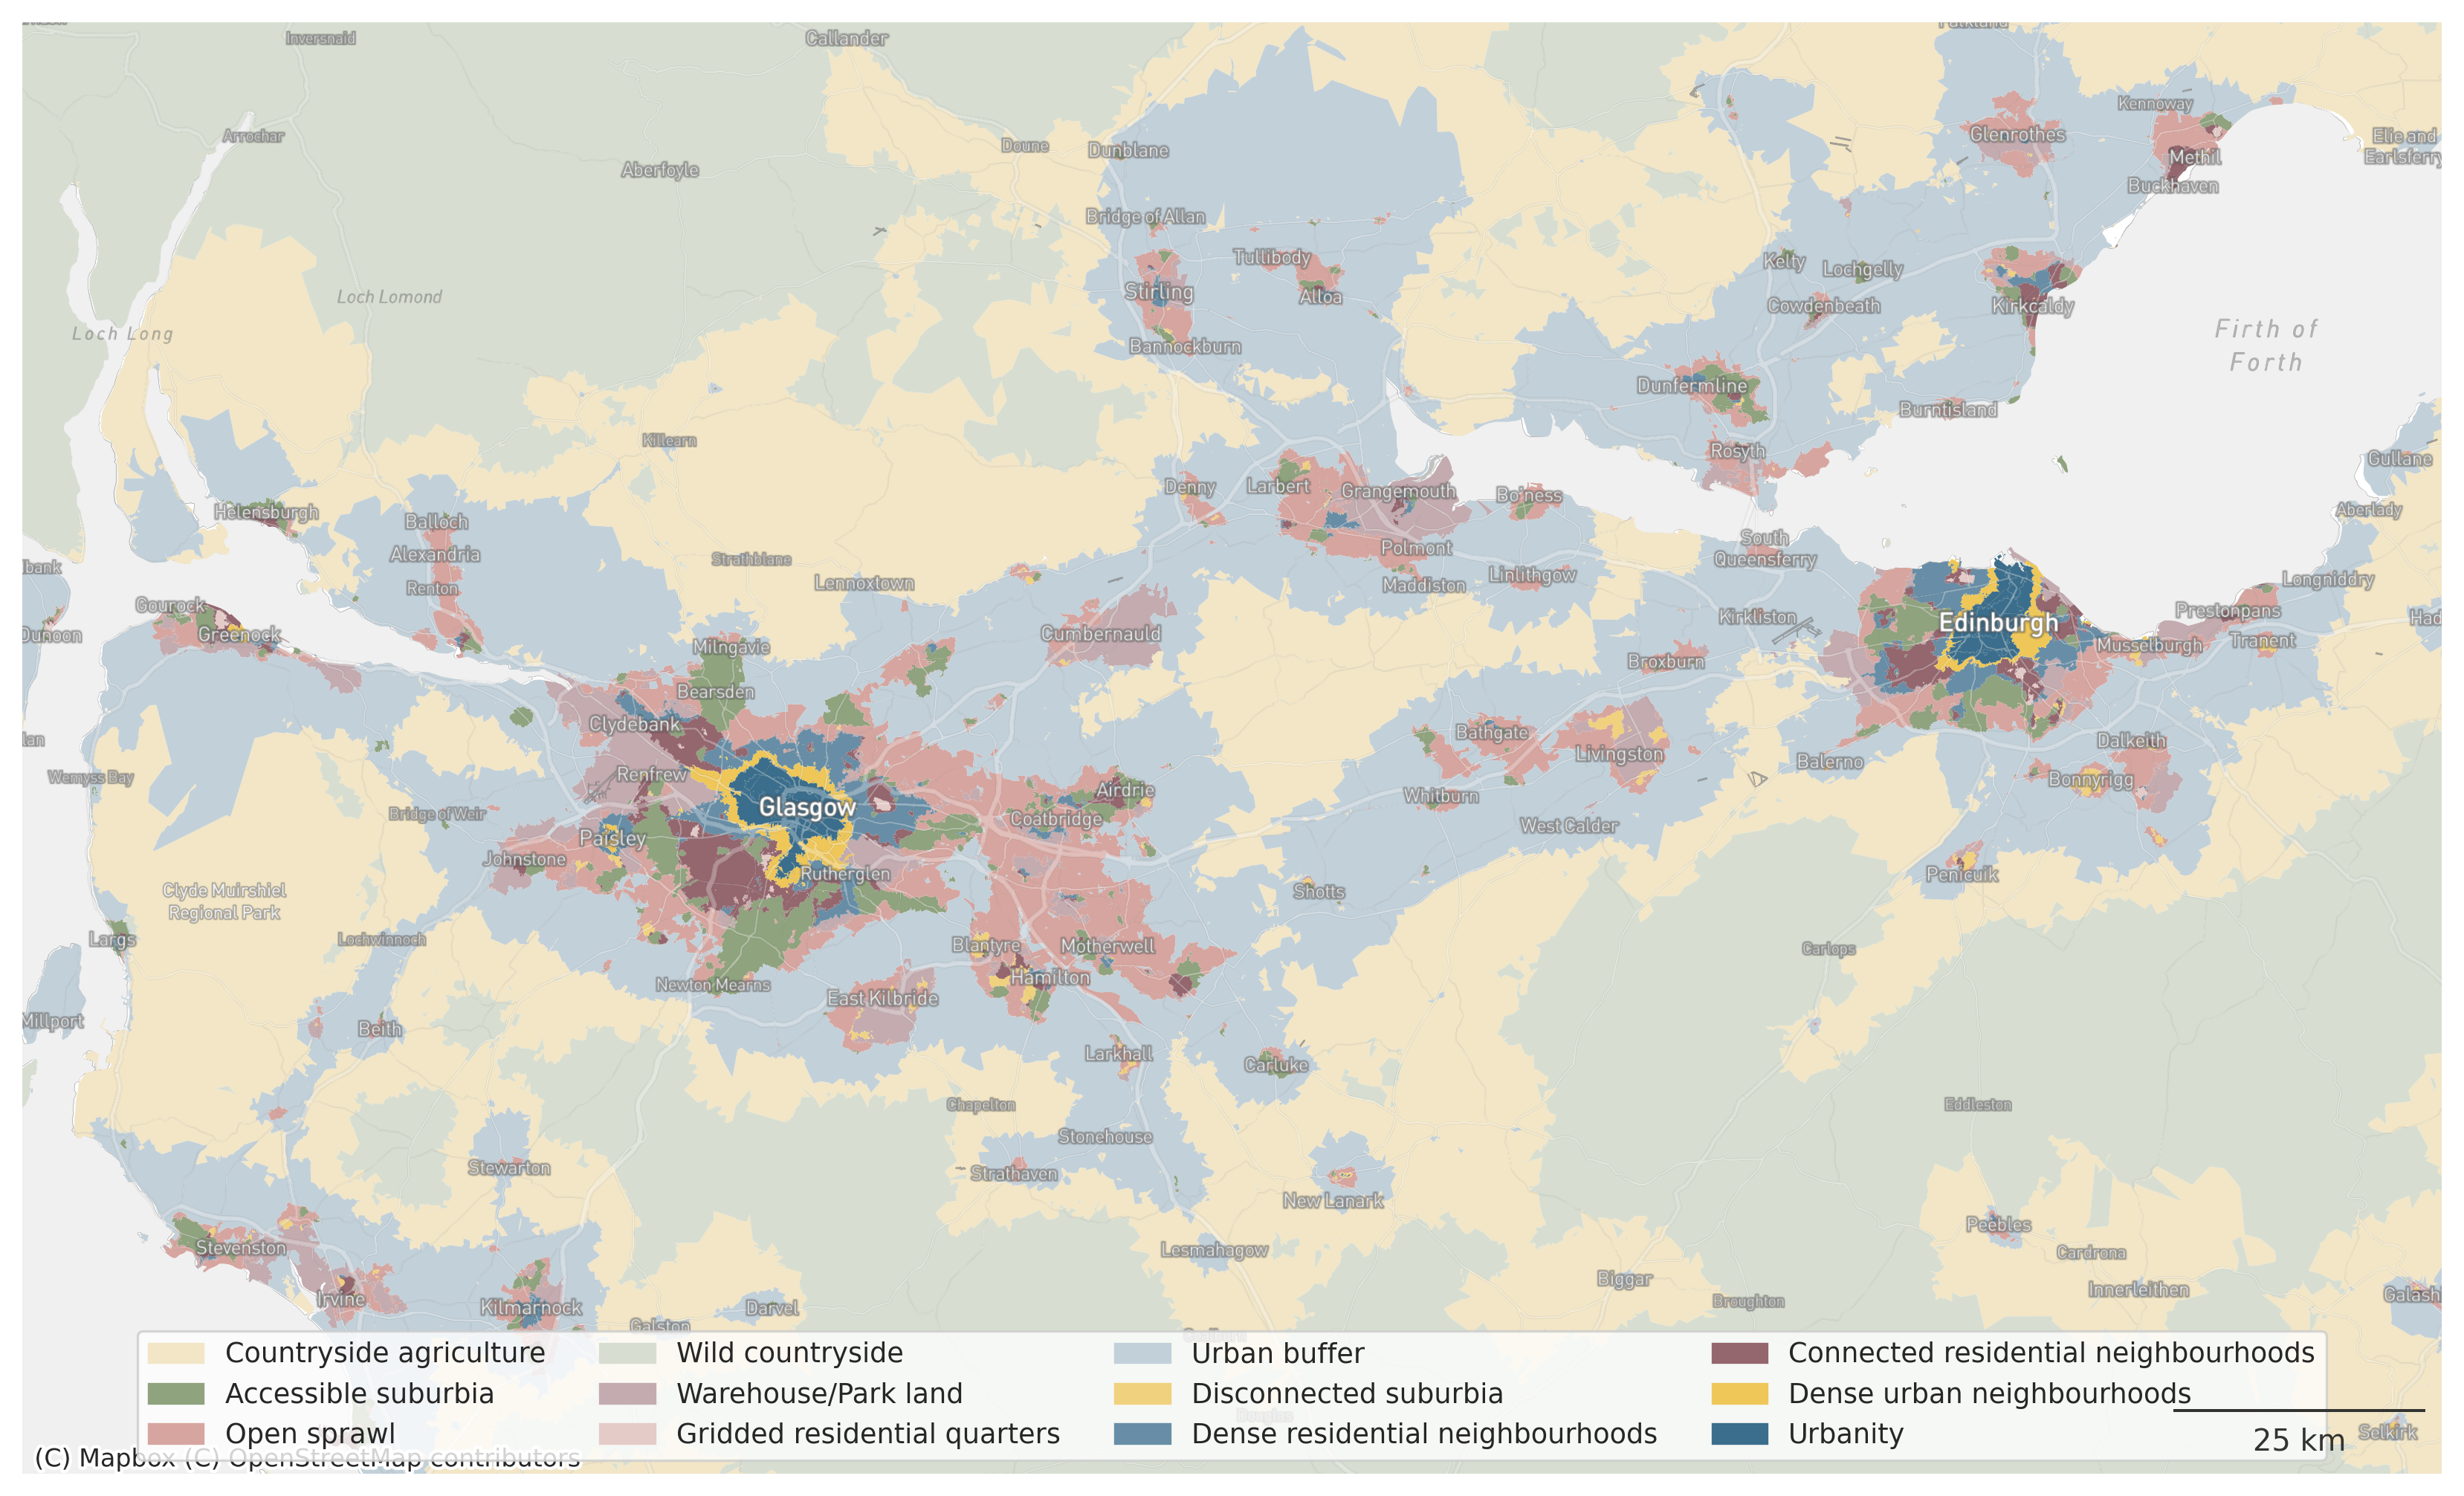
\includegraphics[height=8cm]{fig/signatures_scottish_belt_12_classes.png}
     \end{subfigure}
    \hfill
    \begin{subfigure}[b]{0.19\textwidth}
        \centering
        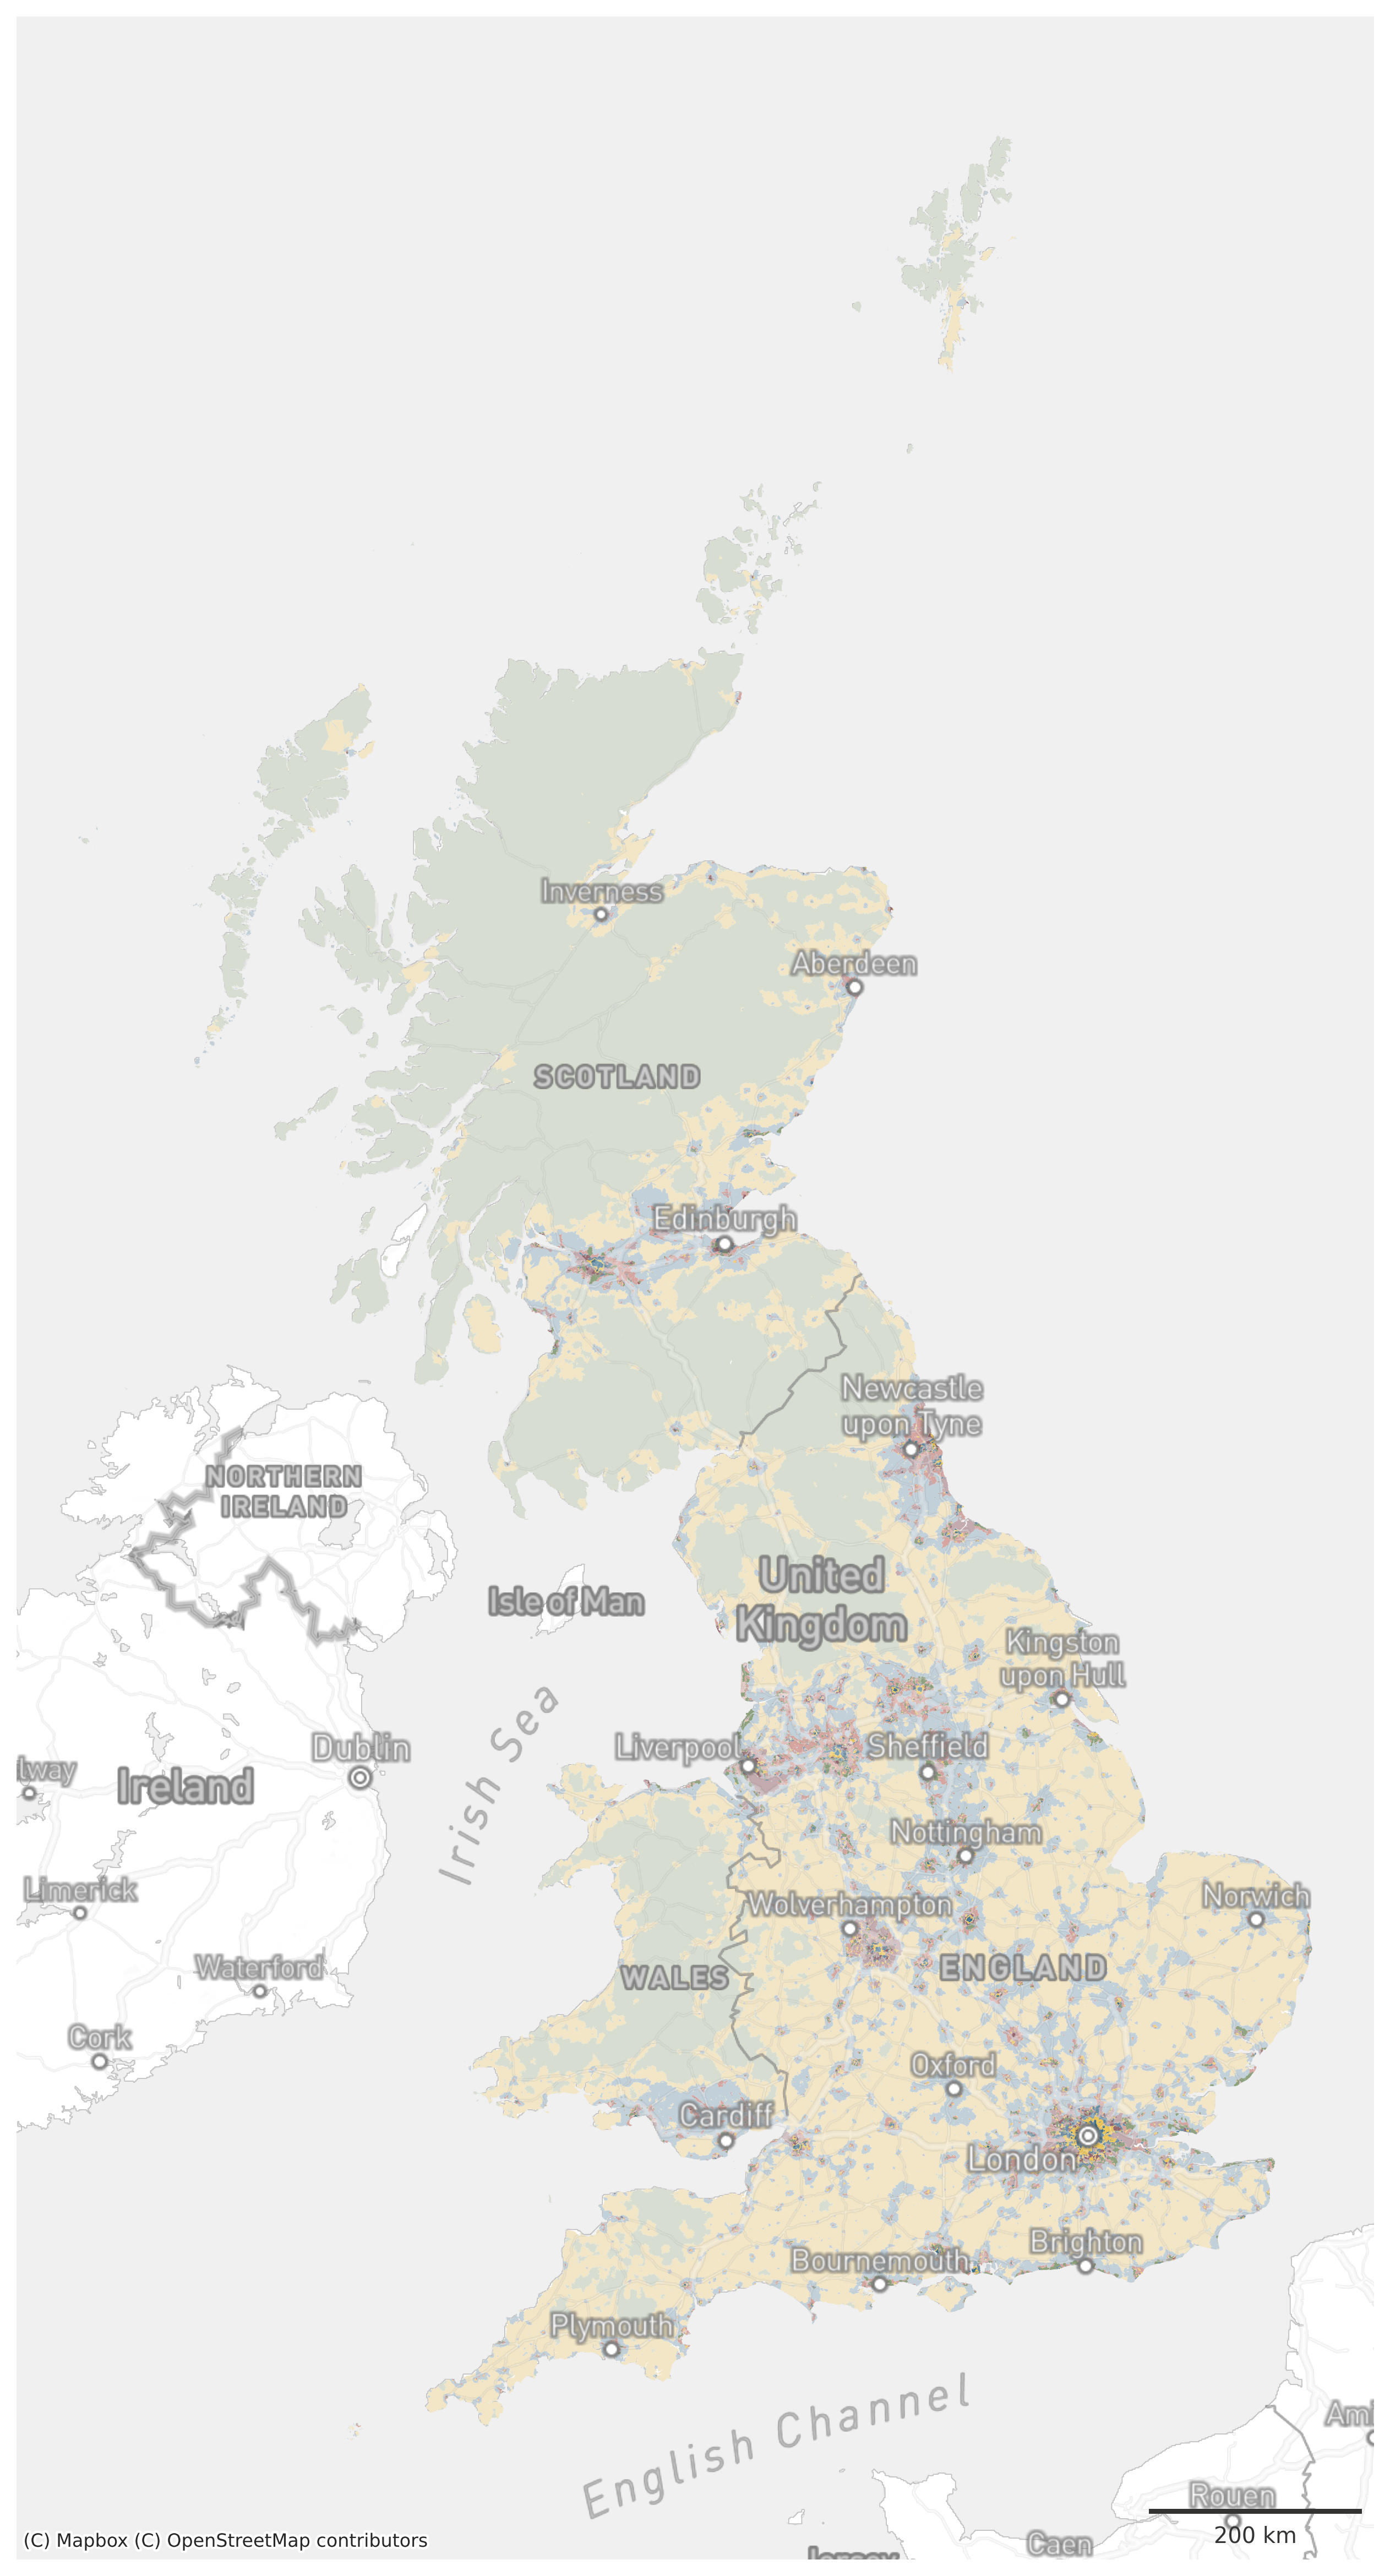
\includegraphics[height=8cm]{fig/signatures_gb_12_classes.png}
    \end{subfigure}
    \caption{Spatial signatures in the full extent of Great Britain (right) and zoomed to a
metropolitan area of the Scottish Central Belt stretching from Glasgow to
Edinburgh (left),
limited to 12 classes used in this paper.}
\label{fig:signatures}
\end{figure}


\subsubsection{Sentinel 2 imagery}

% 250 words

The second data input used in this research is satellite imagery provided by the
Sentinel 2 mission. Specifically, we use the pre-processed cloud-free mosaic of Sentinel
2 released by \cite{CORBANE2020105737}.
The mosaic provides pixel-level composite based on imagery for the period January 2017-
December 2018 at an original resolution of 10 meters per pixel. While Sentinel 2
captures many spectral bands beyond traditional visible red, green and blue (RGB), this
research uses only RGB bands due to its employment of pre-trained neural networks
stemming from non-satellite imagery that is composed only of RGB and an attempt to
minimize training from scratch that would need to happen to derive weights for other bands. The exclusion of other
bands may be seen as a limiting factor of the work, but we believe that, as with other
aspects that will be discussed later, it efficiently illustrates the \textit{lower
bound} of the performance of the presented method and can be only improved with the addition of
other spectral bands or other data (e.g. synthetic-aperture radar imagery).

Another notable aspect of the Sentinel 2 imagery is the resolution. Ten meters per pixel
may be enough to distinguish LULC classes, as shown by the examples discussed
above. However, it is unclear whether it is enough to delineate types of urban
environments. Individual buildings often do not stretch beyond the spatial extent of two
pixels, which is severely limiting what we can \textit{see} on the image, as illustrated
in Figure \ref{fig:chips}. While other data sources may provide better
resolution\footnote{For example, commercial imagery by Maxar reaches a resolution of
30cm per pixel and imagery by Planet of 50cm per pixel}, potentially improving model
performance, this research is bound within the limits of \textit{open data}, where
Sentinel 2 is the best offering to date.


\subsection{Methods}

% 250 to explain the overarching experiments

We define our challenge as an image classification task and use competing alternatives
to explore which one performs best and to assess whether the \textit{best} is good enough.
Each of them implies geographically relevant
trade-offs. First, we build and train a model composed of a convolutional neural network
and probability modelling able to predict the 12 classes derived from the spatial
signatures. Second, we use methods designed to unveil which of the inherently
geographical decisions being tested has a significant effect on the resulting
performance and should therefore be considered when applying CNN to spatial
problems.

When selecting the CNN architecture, we have intentionally excluded image
segmentation. While it seems like an ideal candidate for the task at hand, there are
several reasons for its exclusion. The first has to do with the spatial signatures and the
nature of the boundaries between individual types. While the dataset from
\cite{fleischmann2022geographical} delineates them with hard boundaries when one cell
is a type A and the neighbouring one a type B, the reality is not that simple, and these
boundaries should be treated more as a fuzzy edge that the hard one. There is very rarely an immediate
switch between one type of urban environment and the other one. In many cities, two
types tend to form a transition on the edges where neither is dominant. A situation like
this is very challenging for the image segmentation as it often looks at delineation of
water bodies, buildings or other precisely defined patches on an image. The second reason is that the image
segmentation, having a prediction for individual pixels, would not allow us to use the
second part of the method and test the effect of spatial lag in modelling efficiently. The only
way of doing that would be to run the experiment on a pixel level which would be
extremely computationally expensive, hence challenging to reproduce. We believe that the
method that can be run on a local machine is in the end, more valuable than the one
requiring a high-performance cluster.

Overall, our exercise is structured as a comparison of models that attempt to
predict the 12 spatial signatures entirely from Sentinel 2 imagery. Each model 1) takes
a set of training data as input; 2) runs the class prediction using the convolutional neural
network (CNN); and 3) builds a (spatial) model on top of the resulting probabilities. The
differences between the models are capturing the geographical options that are being tested:
extent of the area sampled from the satellite imagery into a single \textit{chip},
presence of spatial augmentation, class exclusivity within each chip, and an
architecture of probability modelling on top of a prediction coming from the CNN.
Finally, the performance of each model is assessed using both traditional non-spatial
techniques used in deep learning and bespoke spatial metrics. Given a large number of
resulting values, a regression approach is used to determine the effect of the tested
options.
Each of the steps is further discussed in detail in the subsequent sections.

\subsubsection{Chip size}

% 500 words

The first question that needs to be answered when trying to apply a classification
algorithm on satellite imagery that spans a large amount of continuous land is how
to sample such data into individual patches (or, hereafter, chips)
that can be assigned to classes. Pre-trained CNNs usually expect a square image of
a certain size, but that does not mean that the same size (in terms of pixels) needs to
be directly sampled from the image, thanks to possible resampling. What should be
retained, though, is the ratio. Therefore, we need to sample square chips of a
custom size. Within an image classification framework, which is the first type of model that is tested, we assume that
each chip contains data of a single class only. Therefore, such a chip should be entirely
within the boundary of a single signature type. That poses some restrictions as spatial
signatures, especially in the urban context, tend to be relatively granular, and large chips
would not fit inside the boundaries, reducing the number of
valid chips for training. Therefore, the goal is to find a balance
between the number of chips sampled from the data and the amount of
information each chip can hold. Given the relatively coarse resolution of Sentinel 2, a
chip of 100x100 meters consists of only 10x10 pixels, which may not be enough to capture
the nature of a signature type and distinguish it from other types. On the other hand, a
chip of 1000x1000 meters, which is likely large enough to capture the difference, will
not fit in most of the signature boundaries and we would end up with only a few chips per
urban class.

The literature rarely discusses the decisions involved in defining the chip
size for single-class chip classification. In some cases, the size is predetermined due to the requirement of either a
pre-trained model or an existing set of labelled data \citep{taubenbock2020}. In
others, the size that has
been used in previous studies is applied again without discussing the implications
of such a decision \citep{wang2018mapping}. From a spatial analysis
perspective, this approach is surprising as deciding the chip size is a prime example of the
modifiable areal unit problem (also known as MAUP,
\citealp{openshaw1981modifiable}), especially the aspect about scale, which states that
a change of the scale may affect the outcome of an experiment. Hence such an effect
should be at least considered in an interpretation if not minimized where possible.

In this work, we try to understand the effect of chip size by testing all the models
based on four different chip sizes - 80, 160, 320 and 640 meters representing chips of
8x8, 16x16, 32x32 and 64x64 pixels, respectively, illustrated on a Figure \ref{fig:chips}
and a Supplementary Figure \ref{fig:chip_fits}.


\begin{figure}
    \centering
    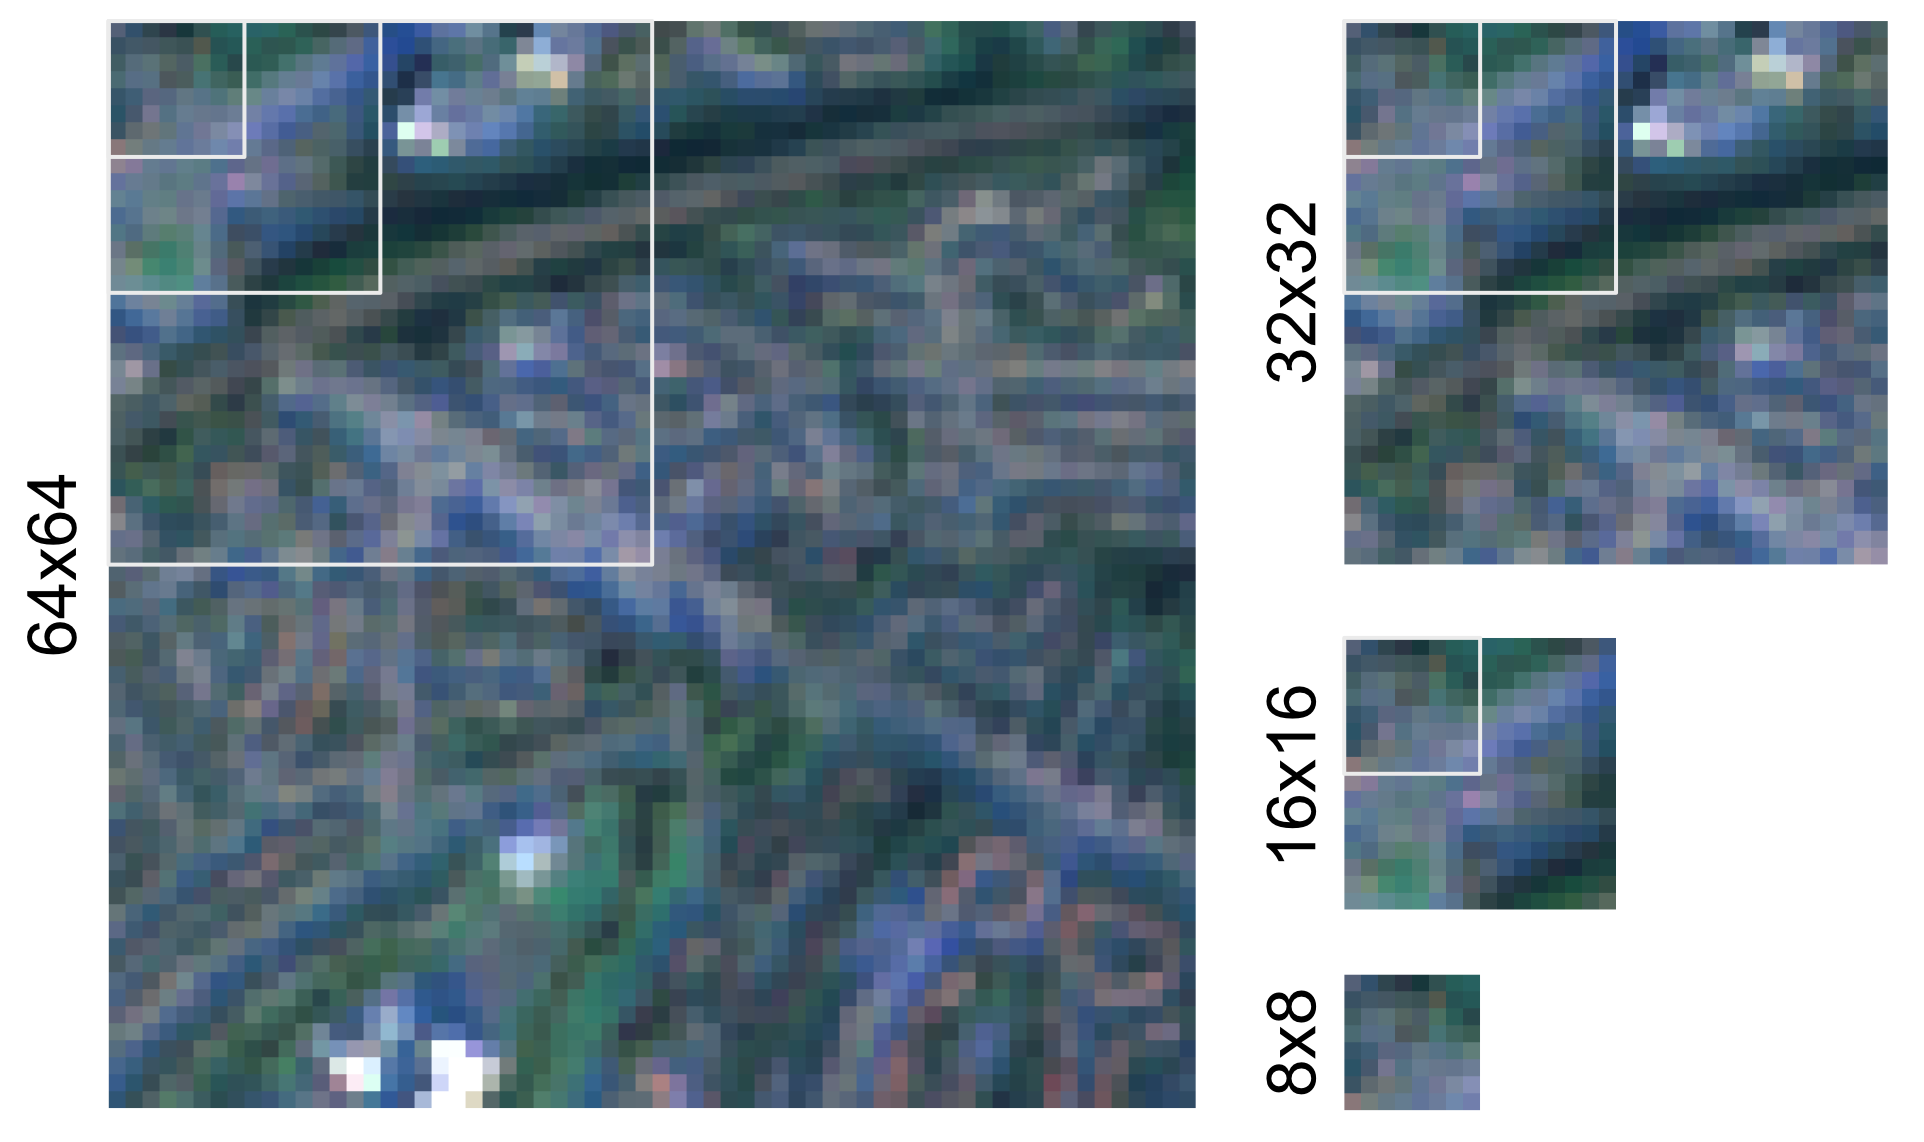
\includegraphics[width=.8\linewidth]{fig/chips.png}
    \caption{Illustration of the selected chip sizes using the Sentinel 2 cloud-free mosaic. Each of the chips also shows the sizes of the smaller options as a white outline.}
    \label{fig:chips}
\end{figure}



\subsubsection{(Spatial) data augmentation - \textit{Sliding}}

% Sliding

% 250 words

As mentioned above, in combination with the signature geometry and
the requirement to keep chips exclusively within a single class, specific chip sizes may result in
insufficient training data for some signature types causing imbalance in the training set. Under-sampling like this
one can be a serious problem that is not unique to spatial modelling. However,
traditional augmentation methods are not directly applicable here. For example, in an
image classification problem trying to determine if there is a cat or a dog on an image,
we add some rotation or zoom to get more versions of
the same image and expand the set of training data. Neither of these methods is
applicable to spatial problems. Rotating the image would break
natural light conditions, while zooming in would change the scale of the urban environment
we attempt to capture. Moreover, distinction between some signature types is partially
in different orientation of streets, rendering rotation-based augmentation counter-productive.

At the same time, the geographical and continuous nature of the data at hand
allows us to use explicitly spatial augmentation techniques such as the one we
call \textit{sliding}.
Sliding can be seen as overlapping sampling. Instead of overlaying a grid of chips over
target geometry and using each pixel only once, we take the initial grid and slide it a
few pixels horizontally and vertically, as illustrated in Figure \ref{fig:sliding}. If
the boundary of a slid chip is fully within a signature geometry, it is added to the
pool of chips to be used. This process is done repeatedly to ensure that each class has
a reasonable amount of chips to work with, while chips from the large signature types
are intentionally undersampled to retain a relative balance between the classes in the training data.

It is to be noted that sliding can cause data leakage (sequences of pixels being
present in both training and validation) if done before splitting the data into
training and validation subsets. Therefore, we first create the initial grid, subdivide
it spatially into four parts (40\% for CNN training, 10\% for CNN validation, 40\% for
probability modelling training, 10\% for probability modelling validation) and apply
sliding within each part to avoid any pixels being shared among chips from different
sets. Subdivision into the four parts is done within each signature geometry to avoid
potential geographical bias.

\begin{figure}
    \centering
    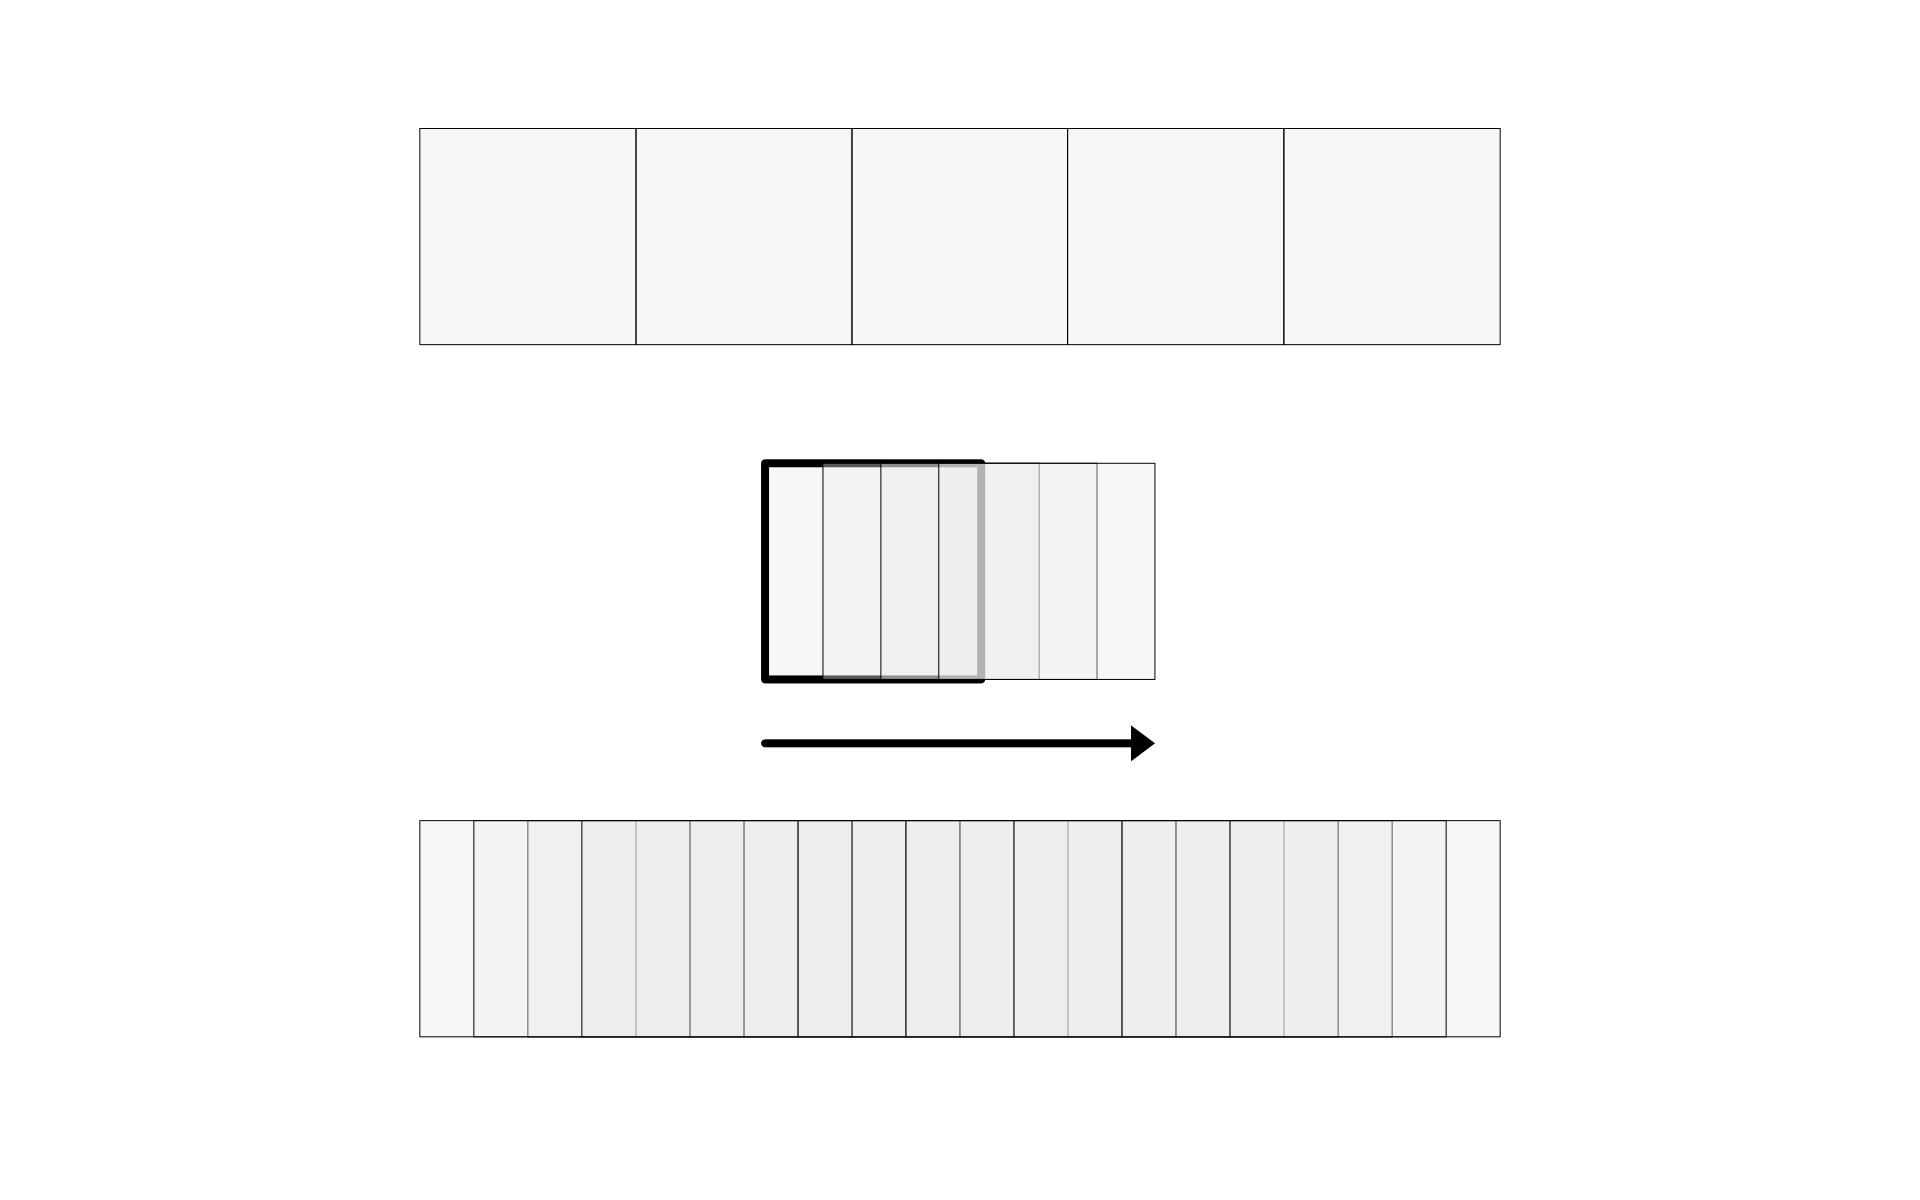
\includegraphics[width=.8\linewidth]{fig/sliding.png}
    \caption{Diagram illustrating the sliding mechanism. The first row shows the initial non-overlapping grid, the last one final overlapping set of chips.}
    \label{fig:sliding}
\end{figure}


\subsubsection{Model architecture}

% 500 words

% Overall content of the section

Model architecture refers to the analytical pipeline that transforms chips
into a prediction for a single signature type. Our competing architectures
contain two main parts. First is a CNN that transforms a single chip into a
set of 12 probabilities, one for each signature type.
Second is a mathematical function that converts such probabilities (
considering only those for the chip of interest or in conjunction with
those of neighbouring chips) into a
prediction for a single signature type. This section describes each of these in detail.
We would like to highlight that, contrary to the majority of deep
learning-focused research, our focus is not on the architecture of the CNN
itself. We assume the effect of geographic choices will largely show similar
behaviour irrespective of the network architecture. For that reason, throughout
our experiments we use \texttt{EfficientNetB4} \citep{https://doi.org/10.48550/arxiv.1905.11946}, pre-trained
on the popular ImageNet dataset \citep{deng2009imagenet}. Appendix \ref*{sec:appendixA} shows a brief comparison of
several standard neural network architectures and their performance on a subset of data
to motivate our decision. We then apply transfer learning by re-training the
top layer of the pre-trained model and replacing it by a
custom sequence of dense layers described below.

% Standard image classification
We consider three variants of the CNN.
The default approach (which we will refer to \texttt{bic}, for ``baseline
image classification'') is a standard image classification problem, using the sets of chips
that are fully within a single signature type. The custom top layer of the pre-trained CNN then contains a Global Average
Pooling (2D) layer, a dense layer with ReLu activation and 256 neurons, and a dense
layer with the softmax activation and a number of neurons equal to a number of classes
(12). The result for a single chip is a collection of 12 probabilities
of a chip belonging to each signature type. The sum of all probabilities is
one.
An extension of this approach (\texttt{sic}, for ``sliding image
classification'') applies this technique to the data being spatially augmented
with the sliding technique described above.

% Multi-output regression
Our third approach recasts the image classification task as a multiclass
prediction. If we relax the requirement that every chip is fully within
the boundaries of a single signature type, we end up with many more available
chips, but now some of them include more than a single label within their
extent. Instead of a single label per chip, we now deal with a 1-D array of them.
This can be beneficial from the geographical perspective as such chips now inherently
encode the co-location of individual signature types and a model could use this information
during the prediction. As signature types usually tend to neighbour only a subset of
other classes (e.g., Urbanity never neighbours Wild Countryside), we can assume that
information on co-location can positively impact predictive performance. We
then include a set of chips sampled from a grid crossing the boundaries of
signature types (using the same chip sizes as before) and adapt the CNN to
perform multi-output regression (\texttt{mor}) instead of image classification. This change
implies the top layer is now composed of a Global Average Pooling (2D) layer, a
dense layer with ReLu
activation and 256 neurons, and a dense layer with the sigmoid activation and a number of
neurons equal to a number of classes (i.e., 12). The result for a single chip is a similar
collection of probabilities, but these are now predicted proportions. As such,
the sum of all of them ranges between 0 and 12 rather than between 0 and 1.

A comparison of the total
number of chips used by each CNN is available in the supplementary table \ref{tab:chip_counts}.
The split of chips is then 40\% for CNN training, 10\% for CNN validation, 40\% for
probability modelling training, 10\% for probability modelling validation equally across all the options.
All CNN models are trained using the following hyperparameters: number of
epochs: 200, optimizer: Adam, patience: 5, and a batch size: 32. See the relevant code
in the linked repository for details.

% Spatial modelling of probabilities TODO: Dani, from this section below are your bits.
The second step in the pipeline takes chip probabilities and turns them into
predictions of a signature type. To do this, we compare five approaches of
differing complexity and sophistication. These five variants stem from the
combination of two components: the set of inputs used to make the prediction and
the function transforming them into a single signature type. For a given chip
$i$, we can express this step of the pipeline mathematically as follows:

\begin{equation}
\begin{split}
        S_i & = f(P) \\
        P & = \underbrace{
                \sum_{k} P_{k-i}
        }_\text{baseline}\;
        \underbrace{
                \left[+ \sum_{k} \sum_j^{N-1} w_{ij} P_{k-j}\right]
}_\text{wx}
        \label{eq:sp_model}
\end{split}
\end{equation}

where $S_i$ is the prediction for the signature type of chip $i$ (one of the
        $k$ available types, where
$k=12$ in our empirical case, see Section \ref{sec:matmet_ss}) and $f(\cdot)$ is a function that
transforms the inputs $P$ into $S_i$. The five
approaches we compare derive from the different implementations of $f(\cdot)$
and $P$. On the latter, we compare models that only use
$P_{k-i}$ (probability that chip $i$ is of type $k$) generated by the CNN for
chip $i$ (\texttt{baseline}) with alternatives
(signalled with the \texttt{wx} term) that, in addition,
also include an average of $P_{k-j}$ (probability that chip
$j$ is of type $k$), which are the
probabilities generated by the CNN for each neighbour $j$ of chip $i$. This is
akin to what in spatial analysis is called the \textit{spatial lag} of each
probability, and is calculated using a spatial weights matrix $W$ that records
the spatial relationship between every chip in the set. In our $W$, two
neighboring locations $i$ and $j$ will receive a weight $w_{ij}=1$,
if they are in the same of the four split sets as defined above, and if they
either are geographically contiguous or are nearest neighbours; while otherwise
they will be considered non-neighbours and receive a weight $w_{ij}=0$. To obtain
an average of the neighbors, we row-standardise $W$ so that $\sum_j w_{ij} =
1$. The second dimension other than $P$ we vary is the function $f(\cdot)$ that maps
it to the prediction $S_i$. We take three distinct approaches here: simply
picking the maximum probability (\texttt{maxprob}), which we only use without the spatial lag of
probabilities; an ensemble of binary logit models to predict each class
(\texttt{logite}), then selecting the class with top probability, which we
also use with the \texttt{wx} variant; and a histogram-based gradient boosted
classifiers inspired by LightGMB \citep{ke2017lightgbm} and implemented in
\texttt{scikit-learn} \citep{pedregosa2011scikit}. This yields our five
competing models:
\texttt{maxprob}, \texttt{logite\_baseline}, \texttt{logite\_baseline-wx},
\texttt{HGBC\_baseline}, and \texttt{HGBC\_baseline-wx}.

\subsubsection{Performance metrics}

% 500 words
The goal of our experiments is to compare different models under varying
geographical conditions to learn both which performs best, but also how
different choices of geographical nature influence the overall performance
when predicting form and function from satellite imagery.
To provide a workbench that systematically compares each model and setup, we
use a set of performance scores that operate either at the global or class level,
and that measure performance in the traditional machine learning sense, as
well as in the spatial sense.

% Traditional non-spatial
We use four standard performance scores. \textit{Cohen's kappa} score ($\kappa$,
\citealp{cohen1960coefficient}) is a measure of agreement between two sets of
categorical labels that ranges from -1 to 1. Intuitively, it measures the
extent to which the two sets agree with each other (i.e., same label for the
same observation) beyond what would be expected from pure chance
($\kappa=0$). Cases where there is more disagreement than expected from chance
receive a negative score. \textit{Global (within-class) accuracy} captures the
proportion of observations correctly predicted (in a given class). The
\textit{Macro F1} is a score that aggregates class-based F1
scores. The F1 is the harmonic mean between precision (proportion of
chips predicted in one class actually belonging to that class) and recall
(proportion of chips belonging to a given class being predicted as such).
We use both the \textit{weighted Macro F1} as well as the \textit{averaged
Macro F1}. The latter takes the standard mean of the F1 scores for each class,
while the former weights each F1 by the proportion of chips in each class.

% Explicitly spatial metrics % Why % Which ones % Why those? (ideally link to Miguel's
%paper suggestions)
In addition to traditional performance scores, we also evaluate how similar
the spatial pattern of predictions is to that of the original labels.
The measures described above are all ``spatially unaware'' in the sense that
they quantify different aspects of the correctness of a model's
predictions but ignore their spatial patterning. Two
sets of results may have the same amount of correct predictions, but in one,
the spatial layout of such predictions may be close to
that of the observed labels, while the other one spatially allocates mispredictions in
a way that differs more from what is observed empirically. Given the nature of
our classification challenge --identify form and
function over space from satellite imagery-- the spatial dimension of model
performance is of great importance. Since the spatial signatures represent a
set of (12) distinct categories, we rely on the \textit{join counts} statistic
(JC, \citealp{cliff1981spatial}). The JC measures the degree of spatial
concentration in a binary categorical variable; hence, we use it at the class
level. For each class in each model, we retain the proportion of pairs of
chips in the same class that are spatial neighbours (``joins'') over the total number of
pairs that are spatial neighbours.
Our neighbourhood definition relies on two alternative spatial weights matrices:
one based on a distance threshold of $1Km$ ($W_{thr}$), and one that combines
the nearest neighbour with those defined by contiguity ($W_{union}$).
Our metric of interest is then the error (i.e., absolute
value of the difference) between this proportion for the model of interest and
that of the observed labels.

\subsubsection{Summarizing experiments}

% 250 words

The setup described above generates over 60 different
models to be trained to predict 12 signature types and six performance measures
to evaluate them. Making sense of their results requires a
systematic approach that summarises them and provides explicit tests for the
questions we are trying to answer. We achieve this goal by fitting linear
regressions that explain performance scores for each model as a function
of the characteristics of the setup evaluated. Specifically, we estimate the
following two equations. First, for global metrics, we run:

\begin{equation}
        Perf_r = \alpha +
        \sum_m \delta_m M_r +
        \sum_a \gamma_a A_r +
        \beta_1 Chip \; Size_r +
        \beta_2 W_r +
        \epsilon_r
        \label{eq:reg_global}
\end{equation}


where $Perf_i$ is each of our four global performance scores measured for trained
model in setup $i$; $\alpha$ is an intercept; $M_i$ are indicator variables for the
type of model we estimate (i.e., \texttt{maxprob}, \texttt{logite},
\texttt{HGBC});\footnote{We remove \texttt{HGBC} to avoid perfect
collinearity and hence treat it as the reference model.} $A_i$ are,
similarly, indicator variables for the architecture used (i.e.,
\texttt{bic}, \texttt{sic}, \texttt{mor});\footnote{We remove \texttt{BIC} to avoid perfect
collinearity and hence treat it as the reference model.} $Chip \; Size_i$
captures the number of pixels the chips in the setup contain; $W_s$ is another
indicator variable that takes the value of one if the model includes the
spatial lag of signature type probabilities and zero otherwise;
and $\epsilon_i \sim \mathcal{N}(0, \sigma)$ is an i.i.d. error term.

Second, for class-based scores, we fit:

\begin{equation}
        Perf_{r-s} = \alpha +
        \sum_m \delta_m M_r +
        \sum_a \gamma_a A_r +
        \beta_1 Chip \; Size_r +
        \beta_2 W_r +
        \beta_3 \left[\%\right]Obs_{r-s} +
        \sum_s \zeta_s S_{r-s} +
        \epsilon_{r-s}
        \label{eq:reg_class}
\end{equation}

where $\left[\%\right]Obs$ represents either the number of chips in
signature $s$ in setup $i$ or as a proportion of the total; and $S_{i-s}$ an
indicator variable for the signature type $s$;\footnote{We remove
\texttt{Accessible suburbia} to avoid perfect collinearity and hence treat it
as the reference model.} and the rest is as in Equation \ref{eq:reg_global}.
%
Importantly for both equations,
$\delta_m/\gamma_a/\beta_1/\beta_2/\beta_3/\zeta_s$, parameters to be
estimated by the regression model, provide a direct and formal test to the key
questions we set out to answer with our experiments.


% 3000 words

% Section 3 - Results
\section{Results} % 500 words in total
\label{sec:results}

% Overview of numbers
Global accuracy is shown in the Table \ref{tab:global_accuracy}. It may seem that the
results are underwhelming but taking a closer look, it is true only for some models,
usually using smaller chip sizes and simpler architecture. Out of 60 tested models,
14 have global accuracy over 0.5, 6 over 0.6 and one over 0.7. Compared to the relevant
metrics from established LULC models, \citealp{venter2022global} reports that ESRI's
Land Cover reaches global accuracy of .75, Google's Dynamic World 0.71 and ESA's World
Cover 0.65, rendering our highest performing models at par with these. However, they
do perform considerably worse than established LCZ models, that report global accuracy of
0.87 \citep{taubenbock2020}. Yet, this difference is expected as LCZ classes are designed with remote sensing
in mind while spatial signatures aim to reflect the form and function independent of whether
the distinction between two signature types shall be seen from satellite imagery. Nevertheless,
global accuracy is far from providing the full picture.

\martin{The JSON with HistGradientBoostingClassifier 16 BIC is corrupted, so we don't know the value.}

\begin{table}
        \centering
\begin{tabular}{llrrr}
        \toprule
         & Chip Size & B.I.C. & S.I.C & M.O.R \\
        \midrule
        \multirow[t]{4}{*}{maxprob} & 8 & 0.30 & 0.32 & 0.29  \\
        & 16 & 0.27 & 0.35 & 0.28  \\
        & 32 & 0.42 & 0.34 & 0.35  \\
        & 64 & \textit{0.50} & 0.46 & \textit{0.58}  \\
        \cline{1-2}
        \multirow[t]{4}{*}{logite} & 8 & 0.32 & 0.35 & 0.31  \\
         & 16 & 0.36 & 0.36 & 0.31  \\
         & 32 & 0.46 & 0.36 & 0.36  \\
         & 64 & \textbf{0.60} & 0.47 & \textit{0.58} \\
        \cline{1-2}
        \multirow[t]{4}{*}{logite-wx} & 8 & 0.34 & 0.41 & 0.33  \\
         & 16 & 0.42 & 0.46 & 0.33  \\
         & 32 & \textit{0.52} & 0.48 & 0.39  \\
         & 64 & \textbf{0.67} & \textit{0.55} & \textit{0.59} \\
        \cline{1-2}
        \multirow[t]{4}{*}{HistGradientBoostingClassifier} & 8 & 0.32 & 0.36 & 0.32  \\
         & 16 & NaN & 0.37 & 0.33  \\
         & 32 & 0.48 & 0.40 & 0.49  \\
         & 64 & \textbf{0.62} & 0.48 & \textit{\textbf{0.71}}  \\
        \cline{1-2}
        \multirow[t]{4}{*}{HistGradientBoostingClassifier-wx} & 8 & 0.35 & 0.44 & 0.35  \\
         & 16 & 0.44 & 0.47 & 0.34  \\
         & 32 & \textit{0.54}  & \textit{0.50} & 0.40 \\
         & 64 & \textbf{0.68} & \textit{0.56} & \textbf{0.63} \\
        \bottomrule
\end{tabular}
\caption{\label{tab:global_accuracy}\footnotesize Global accuracy of all the models
tested in this study. Values higher than 0.5 are highlighted in italic, values higher than
0.6 in bold and a value over 0.7 in bold italic.}
\end{table}

% figure 1 - within class accuracy per model
Within-class accuracy by the model can be seen in Figure \ref{fig:wc_accuracy_x_model} (a
sister figure where scores are grouped by signature rather than by model can be found in
Appendix \ref{sec:appendixB}). We can notice some consistent patterns already. The
baseline image classification (\texttt{bic}) tends to underperform other architectures,
especially on more urban signature types. On the other hand, multi-output regression (\texttt{mor}),
using the larger chip size (32 or 64), tends to show the highest values across signature
types and models. If we look at accuracy for individual signature types, both extremes
(urbanity on one side and both countryside classes on the other)
tend to be the easiest to predict. Regarding the models, there is no immediate conclusion to be
made apart from a clear indication that the maximum probability (\texttt{maxprob}) approach is generally
worse than any of the modelling, suggesting that there is a value in the modelling step.
The within-class accuracy can be further explored using confusion matrices available as an
Appendix \ref*{sec:appendixC}.

\begin{figure}
    \centering
    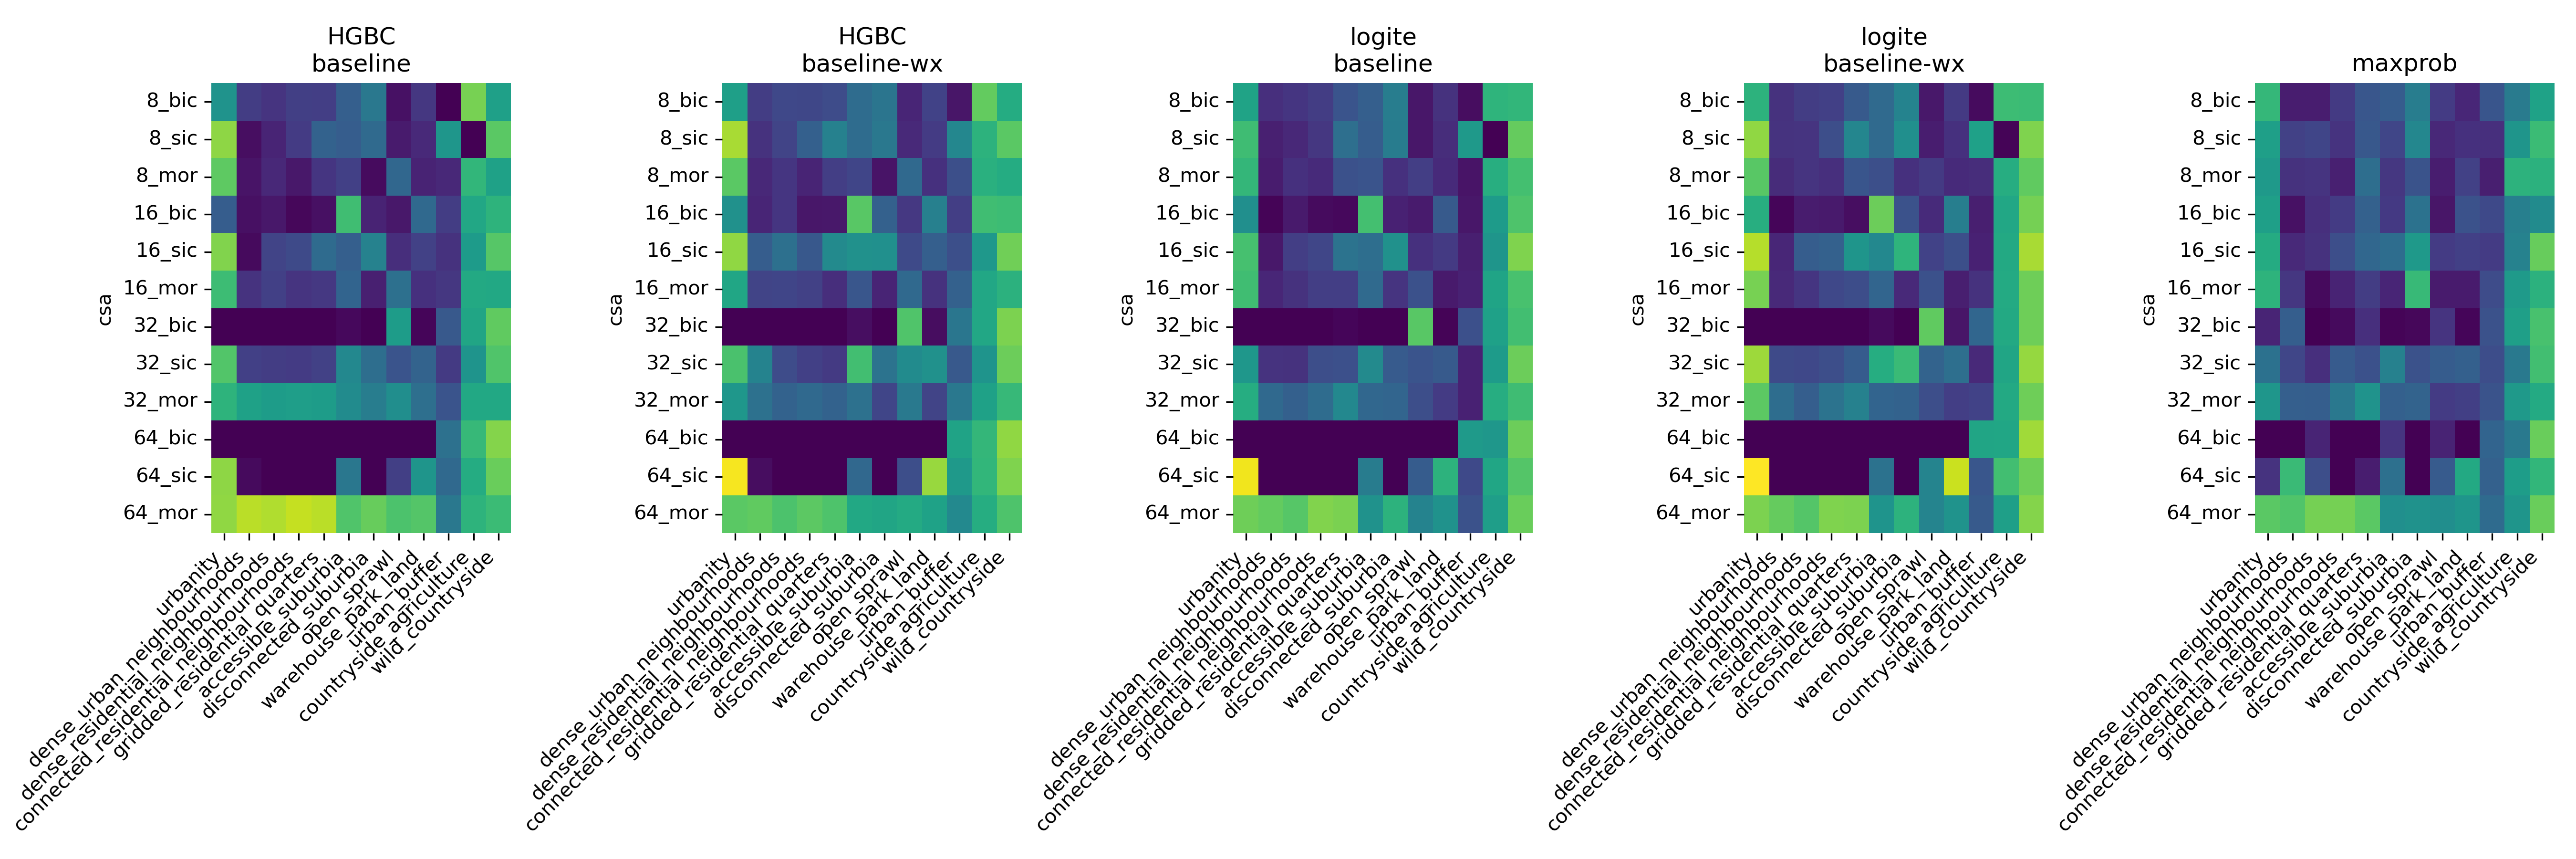
\includegraphics[width=1.0\linewidth]{fig/wc_accuracy_x_model.png}
    \caption{\footnotesize Within-class accuracy scores grouped by model. Each panel
    represents results from one of the five models compared, namely:
    histogram-based boosted classifier (\texttt{HGBC}) with features
    pertaining only to a given chip (\texttt{baseline}) or including also features
    from neighbouring ones (\texttt{baseline-wx}); Logit ensemble
    (\texttt{logite}) with the same two variations; and a simpler maximum
    probability approach (\texttt{maxprob}). Each row in the heatmap
    corresponds to a pair of chipsize (8, 16, 32, and 64 pixels)
    and architechture (baseline image classification, or \texttt{bic}; sliding
            image classification, or \texttt{sic}; and multi-output
    regression, or \texttt{mor}) used in the neural network stage of the
    pipeline. Colouring is standardised across panels and values range from
    0 (dark purple) to 1 (bright yellow).}
    \label{fig:wc_accuracy_x_model}
\end{figure}

Whilst plotting the accuracy is a way to build an intuition about the performance of
individual options, it does not quantify their effects. The linear regressions shown in
tables \ref{tab:non_sp_reg} and \ref{tab:non_sp_reg_wc} provide a better insight. The
first regression explains global performance scores (Cohen's kappa, Global Accuracy, Marco F1
weighted and Macro F1 average). We can draw a few conclusions from this. First, the chip size
seems to have a positive effect on the results, as it is consistently
significant across all metrics. Except for the average macro F1 score, there is a
positive effect of the inclusion of spatial lag in the modelling step (W). Regarding the
CNN step, we do not see a lot of significance but there are indications that sliding
image classification and multi-output regression approaches outperform baseline image
classification. Comparing the probability modelling step, we see an indication that the
maximum probability is the least performant of the options, again suggesting the value
of the modelling.


% table 1 non spatial, one col for regression
\begin{table}
        \centering
\begin{tabular}{lcccc}
\toprule
{} &    $\kappa$ & Global Accuracy & Macro F1 w. & Macro F1 avg. \\
\midrule
Intercept                                         &  0.2185*** &        0.3236*** &    0.2790*** &      0.1798*** \\
                                                  &   (0.0209) &         (0.0175) &     (0.0174) &       (0.0375) \\
(M) Logit E.                                       &    -0.0245 &         -0.0256* &    -0.0324** &        -0.0325 \\
                                                  &   (0.0168) &         (0.0141) &     (0.0141) &       (0.0302) \\
(M) Max. Prob.                                     &  -0.0559** &       -0.0606*** &    -0.0421** &        -0.0296 \\
                                                  &   (0.0222) &         (0.0187) &     (0.0186) &       (0.0399) \\
(A) M.O.R.                                         &     0.0227 &        -0.0357** &     -0.0278* &      0.1787*** \\
                                                  &   (0.0184) &         (0.0155) &     (0.0154) &       (0.0331) \\
(A) S.I.C.                                         &     0.0232 &          -0.0247 &      -0.0171 &      0.1101*** \\
                                                  &   (0.0184) &         (0.0155) &     (0.0154) &       (0.0331) \\
Chip Size                                         &  0.0036*** &        0.0043*** &    0.0048*** &       0.0014** \\
                                                  &   (0.0004) &         (0.0003) &     (0.0003) &       (0.0006) \\
W                                                 &  0.0572*** &        0.0468*** &    0.0531*** &         0.0392 \\
                                                  &   (0.0168) &         (0.0141) &     (0.0141) &       (0.0302) \\
\midrule
$R^2$                                             &     0.7214 &           0.8281 &       0.8514 &         0.4191 \\
$R^2$ Adj.                                        &     0.6899 &           0.8086 &       0.8346 &         0.3533 \\
N.                                                &     60     &           60     &       60     &         60     \\
\bottomrule
\end{tabular}
    \caption{\label{tab:non_sp_reg}\footnotesize Regression outputs explaining
            global non-spatial
    performance scores. Explanatory variables with a preceding (M) and (A)
    correspond to binary variables for the type of model (with histogram-based
            boosted classifier, or \texttt{HGBC}, as the
    baseline) and architecture (with baseline image classification, or
    \texttt{BIC}, as the baseline),
    respectively. Standard errors in parenthesis. Coefficients significant at
    the 1\%, 5\%, 10\% level are noted with ***, **, and *, respectively.}
\end{table}

The table \ref{tab:non_sp_reg_wc} then looks again at the within-class accuracy explaining
what we have seen in figure \ref{fig:wc_accuracy_x_model}. The
multi-output regression consistently outperforms both baseline image classification and
sliding image classification (which shows inconsistent results itself). Chip size has,
again, a positive effect on the performance, while the inclusion of spatial
lag in the modelling also consistently shows a positive impact. As assumed above, the
prediction of signature types on both extremes of the urban-wild range tends to be
easier than classes in between.

\begin{table}
\begin{tabular}{lccc}
\toprule
{}  &       \multicolumn{3}{c}{Within-Class Accuracy} \\
\midrule
Intercept                                         &   0.1866*** &     -0.0237 &    0.0595** \\
                                                  &    (0.0308) &    (0.0311) &    (0.0303) \\
(M) Logit E.                                      &     -0.0125 &     -0.0125 &     -0.0125 \\
                                                  &    (0.0159) &    (0.0141) &    (0.0146) \\
(M) Max. Prob.                                    &     -0.0188 &     -0.0188 &     -0.0188 \\
                                                  &    (0.0211) &    (0.0186) &    (0.0193) \\
(A) M.O.R.                                        &   0.1753*** &   0.2512*** &   0.1753*** \\
                                                  &    (0.0175) &    (0.0163) &    (0.0160) \\
(A) S.I.C.                                        &   0.1202*** &  -0.0783*** &   0.1202*** \\
                                                  &    (0.0175) &    (0.0209) &    (0.0160) \\
Chip Size                                         &   0.0014*** &   0.0041*** &   0.0014*** \\
                                                  &    (0.0003) &    (0.0003) &    (0.0003) \\
1k Obs.                                           &             &   0.0514*** &             \\
                                                  &             &    (0.0036) &             \\
\% Obs.                                           &             &             &   0.0156*** \\
                                                  &             &             &    (0.0013) \\
W                                                 &    0.0365** &   0.0365*** &    0.0365** \\
                                                  &    (0.0159) &    (0.0141) &    (0.0146) \\
(S)Urbanity                                       &   0.2358*** &   0.2022*** &   0.2574*** \\
                                                  &    (0.0349) &    (0.0309) &    (0.0320) \\
(S)Dense urban neighbourhoods                     &  -0.1420*** &  -0.1075*** &  -0.0998*** \\
                                                  &    (0.0349) &    (0.0309) &    (0.0322) \\
(S)Dense residential neighbourhoods               &  -0.1414*** &  -0.0836*** &  -0.0983*** \\
                                                  &    (0.0349) &    (0.0311) &    (0.0322) \\
(S)Connected residential neighbourhoods           &  -0.1306*** &   -0.0726** &   -0.0754** \\
                                                  &    (0.0349) &    (0.0311) &    (0.0323) \\
(S)Gridded residential quarters                   &   -0.0785** &     -0.0127 &     -0.0049 \\
                                                  &    (0.0349) &    (0.0312) &    (0.0326) \\
(S)Disconnected suburbia                          &    -0.0601* &     -0.0103 &     -0.0019 \\
                                                  &    (0.0349) &    (0.0311) &    (0.0324) \\
(S)Open sprawl                                    &   -0.0845** &  -0.0995*** &  -0.1143*** \\
                                                  &    (0.0349) &    (0.0309) &    (0.0321) \\
(S)Warehouse park land                            &   -0.0857** &   -0.0788** &   -0.0817** \\
                                                  &    (0.0349) &    (0.0309) &    (0.0320) \\
(S)Urban buffer                                   &   -0.0828** &  -0.1382*** &  -0.1753*** \\
                                                  &    (0.0349) &    (0.0311) &    (0.0330) \\
(S)Countryside agriculture                        &   0.2236*** &   0.1593*** &   0.1118*** \\
                                                  &    (0.0349) &    (0.0312) &    (0.0334) \\
(S)Wild countryside                               &   0.3876*** &   0.3283*** &   0.2925*** \\
                                                  &    (0.0349) &    (0.0311) &    (0.0330) \\
\midrule
$R^2$                                             &      0.4979 &      0.6087 &      0.5794 \\
$R^2$ Adj.                                        &      0.4857 &      0.5987 &      0.5686 \\
N.                                                &      720    &      720    &      720    \\
\bottomrule
\end{tabular}
    \caption{\label{tab:non_sp_reg_wc}\footnotesize Regression outputs explaining
            within-class accuracy. Explanatory variables with a preceding (M),
            (A) and (S)
    correspond to binary variables for the type of model (with histogram-based
            boosted classifier, or \texttt{HGBC}, as the
    baseline), architecture (with baseline image classification, or
    \texttt{BIC}, as the baseline) and spatial signature (with Accessible
    suburbia as the baseline),
    respectively. Standard errors in parenthesis. Coefficients significant at
    the 1\%, 5\%, 10\% level are noted with ***, **, and *, respectively.}
\end{table}

% figure 2 - map for a single class target/prediction/

%       \begin{figure}
%           \centering
%           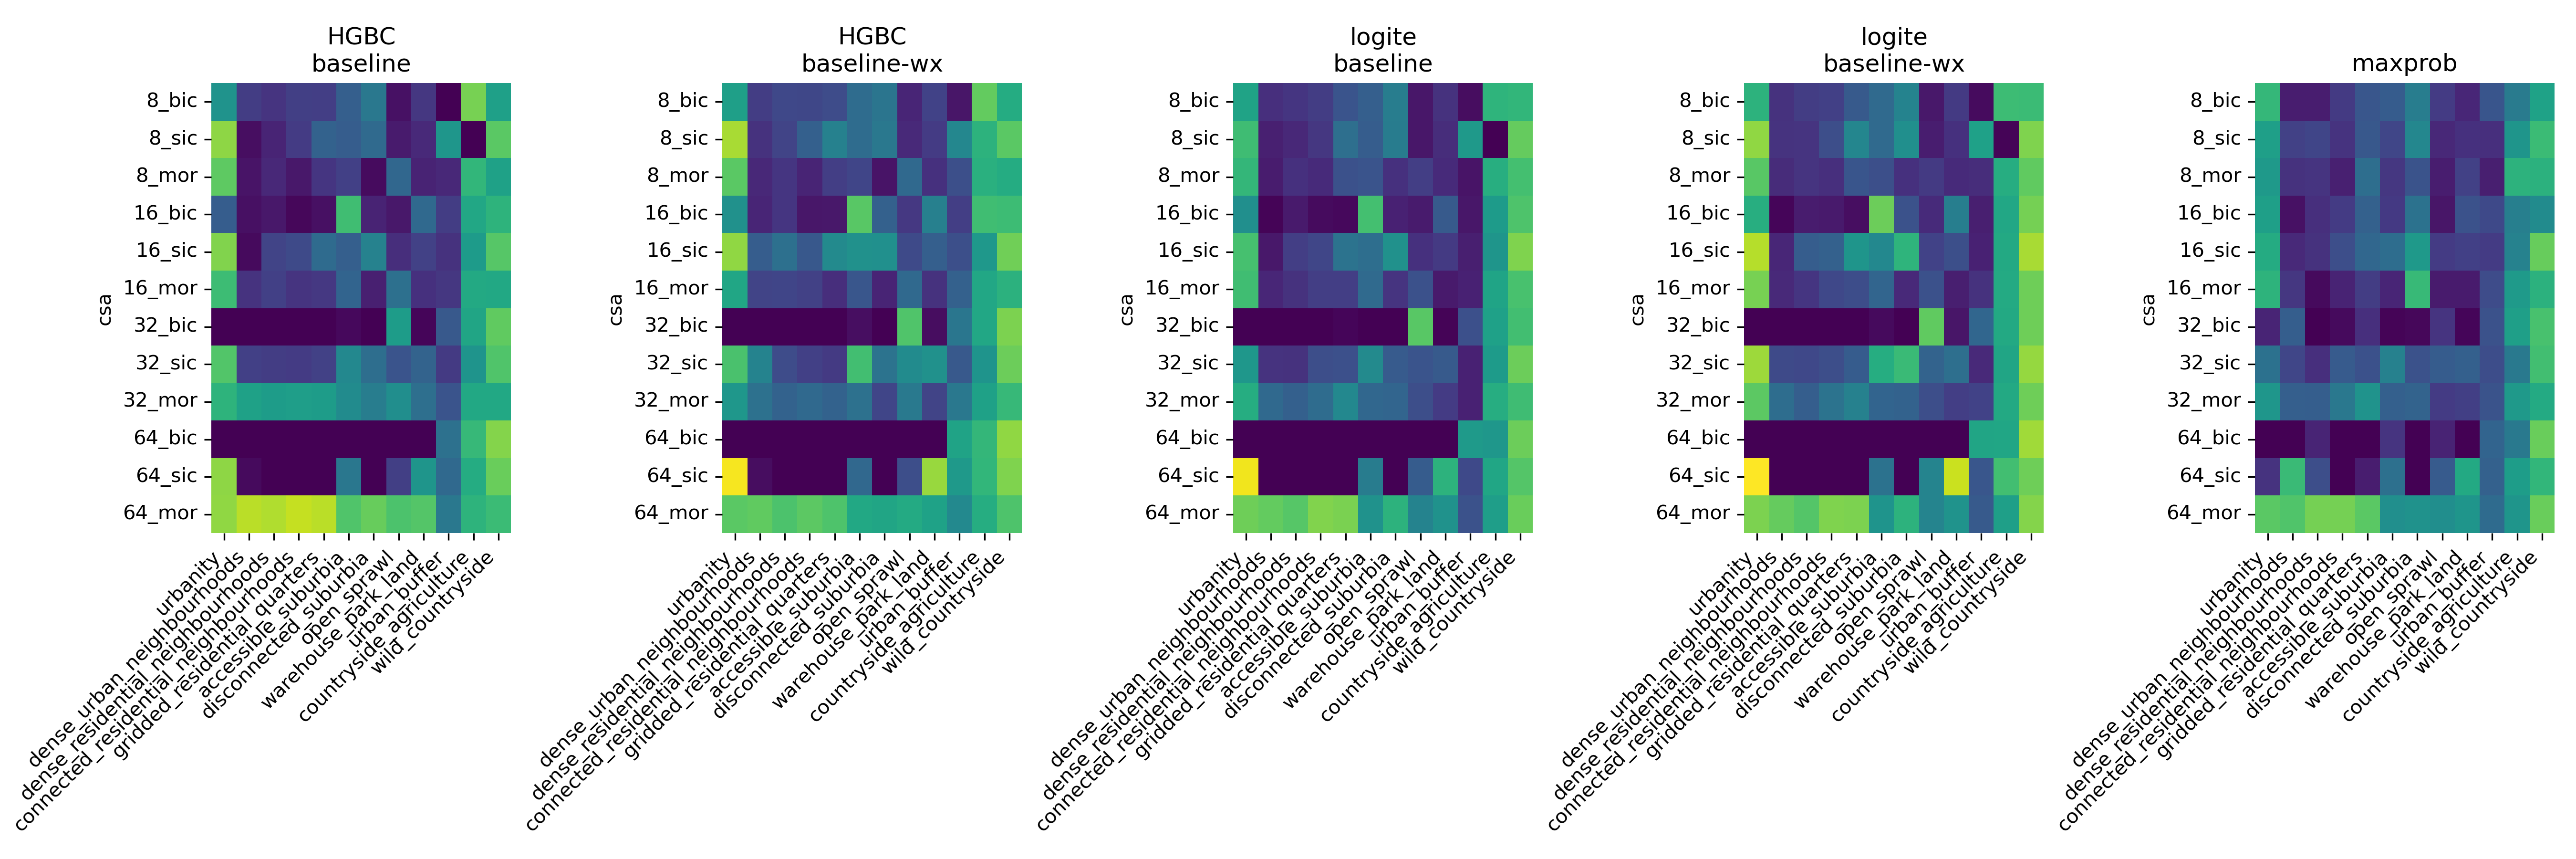
\includegraphics[width=1.0\linewidth]{fig/wc_accuracy_x_model.png}
%           \caption{\footnotesize TBC}
%           \label{fig:prediction_comparison_maps}
%       \end{figure}
% DAB: for space constraints, we have decided to drop it for now

The regression outputs explaining differences in the spatial pattern between observed
and predicted values measured by the Join Counts statistic offer another - spatially
explicit - perspective on the performance of tested model configurations. As such, it
also indicates slightly different results as presented in the table \ref{tab:sp_reg_wc}.
Neither option of the probability modelling steps seem to have a significant effect on
the Join Counts results, unlike in previous performance metrics. However, the
architecture of the neural network step shows a significant effect as multi-output
regression, and in two out of four cases also sliding image classification, outperform the
baseline image classification. While the effect of the chip size is inconsistent across the
options, the inclusion of the spatial lag in the modelling step has a significant effect (at
either 10\%, 5\% or 1\% significance level). The effect of a signature type depends on
its nature. More compact urban types like \textit{Urbanity} and \textit{Dense
urban neighbourhoods} show significance when using a distance threshold spatial weights,
while sparser signature types like \textit{Open Sprawl} and \textit{Urban Buffer} show
significance when using a union of weights.


% table 2 spatial,

\begin{table}
        \begin{tabular}{lcccc}
                \toprule
                {} &  $JC$ & $\log(JC)$ & $JC$  & $\log(JC)$  \\
                {} &  $W\_{thr}$ &  $W\_{thr}$ &  $W\_{union}$ &  $W\_{union}$ \\
                \midrule
                Intercept                                         &   4.3454*** &       1.4617*** &    4.7103*** &         1.6311*** \\
                                                                  &    (0.9507) &        (0.1344) &     (0.5763) &          (0.1080) \\
                (M) Logit E.                                      &     -0.1406 &         -0.0431 &       0.1851 &            0.0481 \\
                                                                  &    (0.4951) &        (0.0700) &     (0.2995) &          (0.0561) \\
                (M) Max. Prob.                                    &      0.1128 &         -0.1223 &       0.2819 &            0.0223 \\
                                                                  &    (0.6442) &        (0.0911) &     (0.3887) &          (0.0728) \\
                (A) M.O.R.                                        &  -3.1630*** &      -0.5744*** &   -2.7875*** &        -0.4647*** \\
                                                                  &    (0.5494) &        (0.0777) &     (0.3301) &          (0.0619) \\
                (A) S.I.C.                                        &      0.0119 &      -0.2390*** &    -0.6666** &           -0.0481 \\
                                                                  &    (0.5532) &        (0.0782) &     (0.3329) &          (0.0624) \\
                Chip Size                                         &   0.0297*** &         -0.0005 &      -0.0061 &        -0.0080*** \\
                                                                  &    (0.0108) &        (0.0015) &     (0.0065) &          (0.0012) \\
                W                                                 &    -0.9325* &       -0.1376** &   -0.9556*** &        -0.1785*** \\
                                                                  &    (0.4945) &        (0.0699) &     (0.2991) &          (0.0560) \\
                (S)Urbanity                                       &   4.6650*** &       0.6574*** &       0.1156 &           -0.1258 \\
                                                                  &    (1.0696) &        (0.1512) &     (0.6460) &          (0.1211) \\
                (S)Dense urban neighbourhoods                     &     1.7796* &       0.5094*** &       0.7480 &            0.1609 \\
                                                                  &    (1.0695) &        (0.1512) &     (0.6487) &          (0.1216) \\
                (S)Dense residential neighbourhoods               &     -0.8545 &          0.0672 &      -0.4636 &           -0.0920 \\
                                                                  &    (1.0958) &        (0.1550) &     (0.6647) &          (0.1246) \\
                (S)Connected residential neighbourhoods           &     -0.3656 &          0.1543 &      -0.4388 &           -0.1447 \\
                                                                  &    (1.1018) &        (0.1558) &     (0.6647) &          (0.1246) \\
                (S)Gridded residential quarters                   &     -0.2000 &          0.1009 &      -0.6203 &          -0.2111* \\
                                                                  &    (1.0744) &        (0.1519) &     (0.6517) &          (0.1221) \\
                (S)Disconnected suburbia                          &     -0.9752 &         -0.1719 &      -1.0303 &        -0.3358*** \\
                                                                  &    (1.1213) &        (0.1586) &     (0.6684) &          (0.1252) \\
                (S)Open sprawl                                    &     1.8342* &          0.1734 &    2.1575*** &         0.3576*** \\
                                                                  &    (1.0604) &        (0.1499) &     (0.6432) &          (0.1205) \\
                (S)Warehouse park land                            &      0.5496 &          0.2123 &      1.2245* &          0.3054** \\
                                                                  &    (1.0694) &        (0.1512) &     (0.6487) &          (0.1216) \\
                (S)Urban buffer                                   &     -0.0558 &         -0.0931 &    2.7027*** &         0.5164*** \\
                                                                  &    (1.0521) &        (0.1488) &     (0.6382) &          (0.1196) \\
                (S)Countryside agriculture                        &     -1.3759 &        -0.2511* &       0.6623 &            0.0670 \\
                                                                  &    (1.0521) &        (0.1488) &     (0.6382) &          (0.1196) \\
                (S)Wild countryside                               &    -2.0183* &      -0.5065*** &      -0.5918 &           -0.1635 \\
                                                                  &    (1.0521) &        (0.1488) &     (0.6382) &          (0.1196) \\
\midrule
                $R^2$                                             &      0.1589 &          0.1954 &       0.2118 &            0.2660 \\
                $R^2$ Adj.                                        &      0.1368 &          0.1743 &       0.1913 &            0.2468 \\
                N.                                                &      665    &      665        &   670        &     670           \\
                \bottomrule
                \end{tabular}
    \caption{\label{tab:sp_reg_wc}\footnotesize Regression outputs explaining
            (log of) differences in the spatial pattern between observed and predicted values,
            as measured by the Join Counts statistic. The Join Counts for each signature were computed
            using two types of spatial weights: one based on a distance threshold of 1Km ($W\_{thr}$),
            and another one built as a the union of nearest neighbor and queen contiguity matrices ($W\_{union}$).
            Explanatory variables with a preceding (M), (A) and (S)
    correspond to binary variables for the type of model (with histogram-based
            boosted classifier, or \texttt{HGBC}, as the
    baseline), architecture (with baseline image classification, or
    \texttt{BIC}, as the baseline) and spatial signature (with Accessible
    suburbia as the baseline),
    respectively. Standard errors in parenthesis. Coefficients significant at
    the 1\%, 5\%, 10\% level are noted with ***, **, and *, respectively.}
\end{table}


% 500 words

% Section 4 - Discussion
\section{Discussion and conclusion} % 500 words in total
\label{sec:discussion}

% Summarise results
The results can be summarised in four dimensions.
%% Architecture dimension (BIC, SIC, MOR)
The first dimension tested is the way of chip sampling and related CNN architecture.
It seems clear that the baseline image classification is limited, and either the
sliding approach to minimise the disbalance of sample size per class or multi-output
regression shall be preferred in a use case like signature detection. Of the two,
multi-output regression even seems to be better, and one of the reasons could be its
ability to implicitly capture co-location. While BIC and SIC-based models have no
information on
the geographical relationship between neighbouring signature types, MOR directly
captures these as chips often cross multiple signature types. This behaviour is unique
to geographical problems. Aspatial image classification tasks are not able to encode
\textit{distance} between two types in this way. Still, sliding significantly improves the
performance when considering the global Macro F1 score and within-class accuracy, making
it a viable option if we want to stick to the traditional image classification approach.

%% Chip size dimension
The second dimension is the chip size. Except for Join Counts statistics, we see a positive
relationship between model performance and the extent our chips cover. This is an expected
outcome as the larger the chip is, the more information it contains. However, we cannot
blindly follow \textit{larger is better} logic as signature types are composed of
granular geometries, and we see a sampling issue when the chip size grows. While that
can be partially mitigated by using MOR for single-class prediction, it needs to be considered in model
architecture. The results do not suggest that one of the options is the \textit{sweet spot}
of the balance between sample size and amount of within-a-chip data.

%% Modelling dimension
Another dimension looks at the value of modelling on top of probabilities coming from
neural networks. The results indicate that there is value in the modelling step as the
maximum probability option, used as a default if no modelling is employed, tends to
underperform both logit models and histogram-based gradient
boosted classifiers. While the difference between logit and HGBC is not always
significant, some results suggest that the non-linear nature of HGBC provides better
performance than linear logit models.
%% W dimension
The last dimension focuses on the inclusion of the spatial lag in the modelling step as a
geographically-explicit method of capturing the context of each chip. This has one of
the most consistent effects on performance indicating the models that exclude spatial lag have worse
results than those that include it. Yet again, this step would not be possible in an
aspatial image classification context where two samples have no ``spatial'' distance from each
other hence no spatial weights matrix can be created. This is a clear evidence of the value
of explicitly spatial modelling in this context, and we can only recommend wider adoption of such methods.
% What is the best
Combining all the dimensions, we can assume that the optimal model for the detection of spatial
signatures from Sentinel 2 satellite imagery should define CNN for the multi-output
regression problem based on larger chip size and passing the output to non-linear
probability modelling with a spatial lag component.

% Ability to capture signatures % We can do some nicely, some worse. What is next?
Regardless of global performance, we cannot assume that even the best model will perform evenly across all 12
signature types. The within-class performance metrics indicate that some classes on the
extreme sides of the urban-rural dimension are easier to detect. That is not surprising
as both \textit{Urbanity} and \textit{Wild countryside} signature types are unique,
while the difference between \textit{Dense residential neighbourhoods} and
\textit{Connected residential neighbourhoods} that is visible on the satellite imagery
is much more subtle. It is also common that some of the classes are easier to
distinguish than others (\cite{zanaga_daniele_2021_5571936, karra2021global}). However,
any model deployed for periodical updates of signature classification will have to deal
with this limitation.

% limits
%% Sentinel 2 resolution
%% Chip sample imbalance
%% explain why segmentation is not used and tested
The experiments presented in this article focus on specific target data represented by
spatial signatures. Because the signatures are designed to capture the structure of
urban environments, the behaviour of spatial components in the modelling pipeline may
differ when target data are of a different nature. However, we argue that the principle
still holds in most cases. When the target data has a spatial dimension and a similar
structure to the spatial signatures (e.g. relatively large patches of a contiguous area
belonging to a single class), the explicit inclusion of spatial information in the
modelling pipeline will be beneficial as it directly embeds Tobler's first law of
geography into the model \citep{tobler1970computer}. This is a unique advantage of
geographical problems, unavailable when the task is aspatial. While this assumption is
only theoretical now, we believe that will can be empirically tested in future research.

Since this article is restricted to the use of open data at every step, the best current
resolution of satellite imagery is 10 meters per pixel, as offered by the Sentinel 2
mission. That poses some challenges because such a resolution limits the amount of
information we can capture on a small area and may oversimplify urban environments that
are naturally more granular in their patterns than what 10m can capture. Further
research should explore the performance differences when very-high-resolution
imagery is used instead.

The combination of signatures reflecting small-scale urban types and a relatively coarse
resolution leads to another limitation this work faces - the struggle to sample chips
in a balanced manner. This is most prominent in the baseline image classification
problem, where no pixels are shared among chips and all chips need to be exclusive to a
single signature type. The issue is alleviated by class weights in the neural network
architecture, but such a solution is not optimal.

%% What do we make of it in terms of geography
%%% Reiterate the point on the relevance of geography and how our results
%%% support that view and introduce explicitly-spatial/geographical ways to
%%% improve CV models for spatial imagery
Is geography relevant in image classification problems, then? The results presented
above suggest so. An introduction of explicit geographical methods to improve image
classification models based on spatial imagery proves to be beneficial and makes use of what a
unique - spatial - dimension offers. It requires moving beyond traditionally used
pre-trained models than have no sense of adjacency of individual chips/samples. We need
to take a step towards merging GIS expertise with the one that lies in the field of
AI, often based in departments of computer science rather than geography.

% the extent to which DL can be applied to understand urban environments
We can also conclude that when properly designed, deep learning models have a lot of potential
in characterisation of the composition of urban landscapes, if we want to answer the question
from the introduction. How well they perform varies across different signature types, meaning that
it will also vary across different types of urban environments when other classification than
signatures is considered. Nevertheless, we can foresee a variety of applications of
models of the sort presented and tested in this article. The spatial signatures are based on
a large number of data sources with limited temporal rate of updates (notably census data, updated every 10 years), making it nearly impossible to do yearly snapshots
of classification allowing longitudinal studies of evolution of cities. With the classification
derived from satellite imagery, we can expect to see a much higher temporal resolution,
easily resulting in annual updates, providing a detailed insight into the dynamics of urban
expansion, densification and overall change of the shape of cities. This is a potential
application that is not limited to spatial signatures but can be extended to any
classification of urban environments.


When using openly available satellite data that are currently limited to the resolution
of 10 meters per pixel at best, and classification focusing on primarily urban landscape,
our results show both potential and limits. Accuracy is not far from
that of established LULC models that could be increased in future by expansion of the training
data set and possible inclusion of other available bands (like near-infrared) in the model.
A limitation in decreased performance when it comes to distinction between urban areas that
are neither too dense nor too sparse but show different form and function profiles. It is
either a difference that is not visible on imagery (e.g. more driven by function) or a
limitation of the available resolution and / or training data volume. This issue could have
been primarily driven by the nature of spatial signatures as a classification target, and
it shall be tested on other types of urban classification in the future.

% finish with a very general note on the amount of sat data coming and the need to make
% sense of it
While satellite imagery and neural networks have been around for some time already, we
are just entering the era of an increasing abundance of satellite-based data. What used
to be reserved for national agencies and international consortia is becoming a domain of
commercial subjects. Research in the remote sensing area will face not a lack of
available data but the opposite. We may find ourselves in a situation where a vast
amount of data streams will come our way, but we will struggle to make sense of it. We
believe that the research presented in this article helps in finding our way through.


% 1000 words

\section*{Data and code availability statement}

All the data and code will be available on a public repository with DOI upon acceptance
of the article to ensure anonymity of a double-blind review.

\clearpage

\bibliographystyle{apalike}
\bibliography{refs}

\clearpage

\appendix
\section{Technical appendix}
\label{sec:appendix}

\subsection{Comparison of neural network architecture}
\label{sec:appendixA}

\begin{table}
    \centering
\begin{tabular}{llll}
    \toprule
    architecture & top layer & \# neurons in top layer &       global accuracy \\
    \midrule
    EfficientNetB4 &   Flatten &                    128 &  0.663482 \\
    EfficientNetB4 &   Flatten &                    256 &  0.715764 \\
    EfficientNetB4 &   Flatten &                    512 &  0.697187 \\
    EfficientNetB4 &   GlobalAveragePooling2D &                    128 &  0.723726 \\
    EfficientNetB4 &   GlobalAveragePooling2D &                    256 &  0.715764 \\
    EfficientNetB4 &   GlobalAveragePooling2D &                    512 &  0.727972 \\
        ResnNet50 &   Flatten &                    128 &  0.481157 \\
        ResnNet50 &   Flatten &                    256 &  0.481423 \\
        ResnNet50 &   Flatten &                    512 &  0.522824 \\
        ResnNet50 &   GlobalAveragePooling2D &                    128 &  0.469745 \\
        ResnNet50 &   GlobalAveragePooling2D &                    256 &  0.469745 \\
        ResnNet50 &   GlobalAveragePooling2D &                    512 &  0.526274 \\
           VGG19 &   Flatten &                    128 &  0.708333 \\
           VGG19 &   Flatten &                    256 &  0.675425 \\
           VGG19 &   Flatten &                    512 &  0.692144 \\
           VGG19 &   GlobalAveragePooling2D &                    128 &   0.69931 \\
           VGG19 &   GlobalAveragePooling2D &                    256 &  0.678609 \\
           VGG19 &   GlobalAveragePooling2D &                    512 &   0.67224 \\
    \bottomrule
    \end{tabular}
\caption{\label{tab:app_nns}\footnotesize Comparison of global accuracy of different
architectures of neural network on a sample of data with signature types aggregated into
three classes (centres, periphery, countryside) using the baseline image classification.
EfficientNetB4 with GlobalAveragePooling2D and 256 neurons has been used in the final
experiment.}
\end{table}


\pagebreak

\subsection{Within-class performance by spatial signature}
\label{sec:appendixB}

\begin{figure}
    \centering
    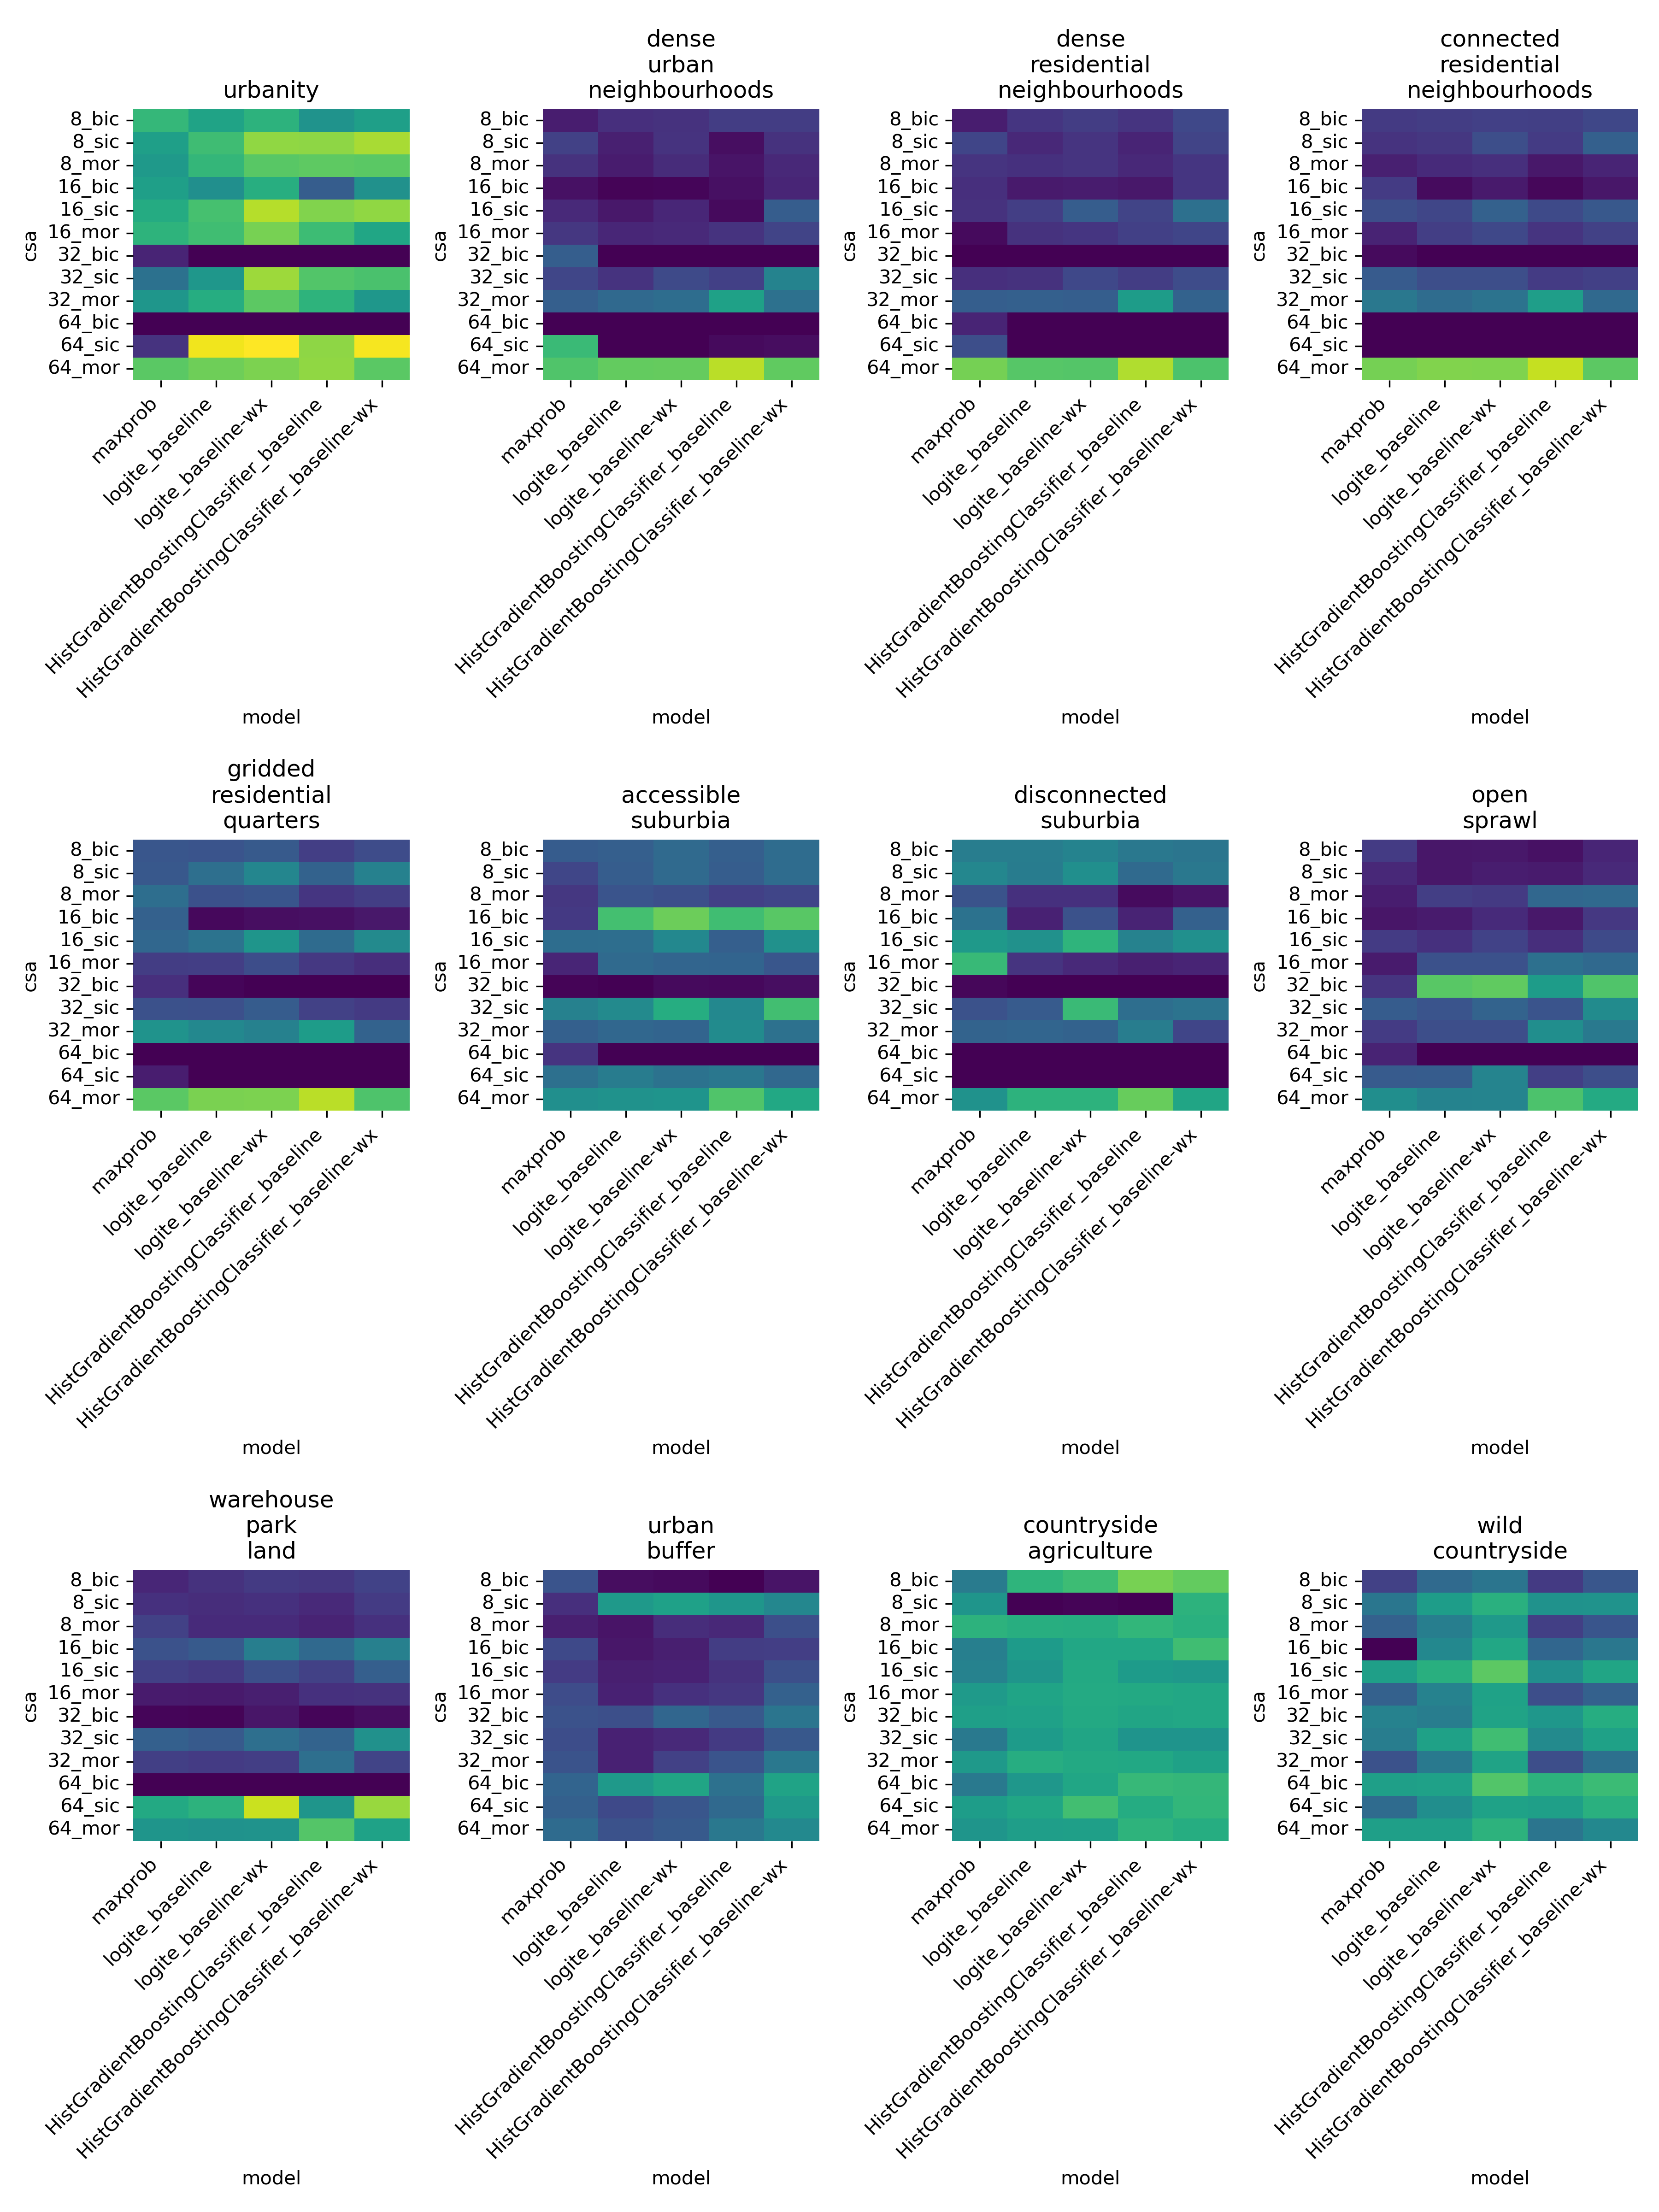
\includegraphics[width=0.8\linewidth]{fig/wc_accuracy_x_signature.png}
    \caption{\footnotesize Within-class accuracy scores grouped by signature. Each panel
    represents results from one of the 12 signatures predicted. Each column in
    the heatmap
    corresponds to one of the five models compared, namely:
    histogram-based boosted classifier (\texttt{HGBC}) with features
    pertaining only to a given chip (\texttt{baseline}) or including also features
    from neighbouring ones (\texttt{baseline-wx}); Logit ensemble
    (\texttt{logite}) with the same two variations; and a simpler maximum
    probability approach (\texttt{maxprob}). Each row
    corresponds to a pair of chipsize (8, 16, 32, and 64 pixels)
    and architecture (baseline image classification, or \texttt{bic}; sliding
            image classification, or \texttt{sic}; and multi-output
    regression, or \texttt{mor}) used in the neural network stage of the
    pipeline.}
    \label{fig:wc_accuracy_x_signature}
\end{figure}

\pagebreak

\subsection{Confusion matrices}
\label{sec:appendixC}


\clearpage

\end{document}
